\chapter{METHODS AND MATERIALS}
\label{chp:methods}

The following methodology aims to compare classical machine learning techniques, ensemble methods, and neural network classifiers in order to assess their average accuracy. Following the initial comparison, the top-performing classifiers will undergo further evaluation against a \gls{cnn} 2D when the responsiveness and effectiveness of these leading classifiers will be analyzed, ensuring that only the most robust and adaptable algorithm is considered for real-world deployment. Similar to other pattern classification tasks, audio classification consists of three essential elements: sensing, audio signal processing, and classification. \textbf{Sensing} involves the measurement of sound events or signals, while \textbf{audio signal processing} focuses on extracting characteristic features from the recorded sound, and \textbf{classification} belongs to the recognition of the contextual information associated with the sound event.

These elements are illustrated in Figure \ref{fig:methodology_illustration} within the \textbf{Training / Classification flow}, which represents the initial stage of the experiment. In the subsequent phase, titled \textbf{Evaluation flow}, similar fundamental elements are encompassed; however, this phase involves real-time simulation using lapel microphones with the selected classifier (winner) embedded in the Raspberry Pi module, with the objective of verifying and confirming the findings obtained during the initial experiment but at this stage under driving conditions. 

\begin{figure}[htbp]
    \raggedright
        \caption{Illustration of the implemented methodology.}
        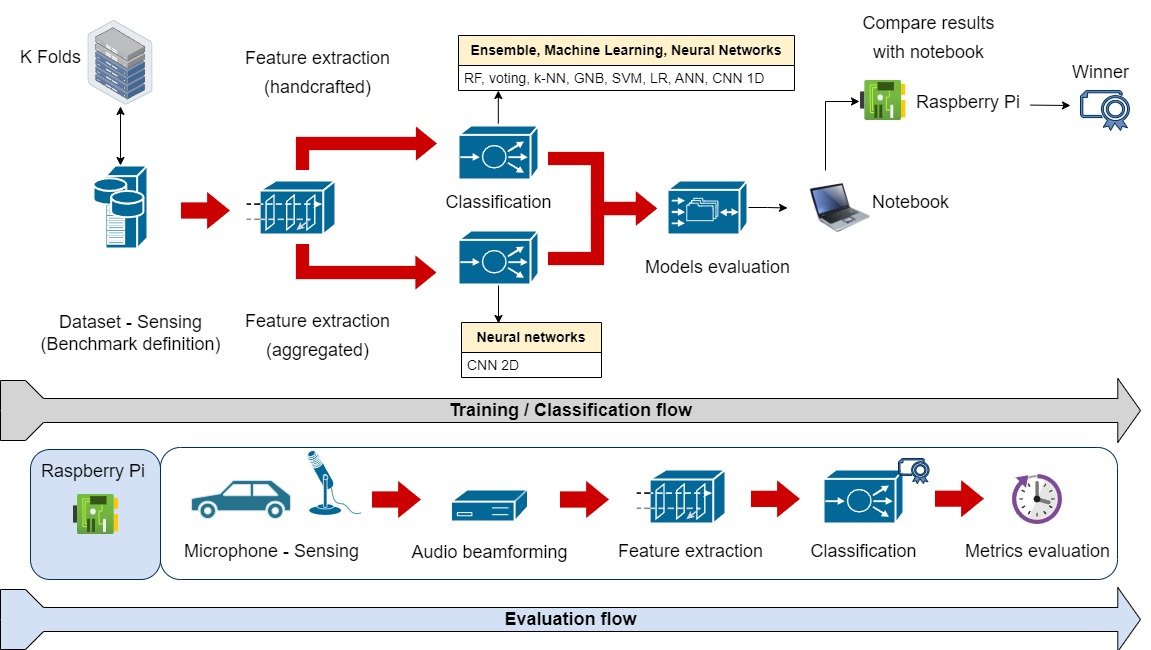
\includegraphics[width=.95\textwidth]{resources/images/050-methods/Methods_diagram.jpg}
        \smallcaption{Source: Author}
        \label{fig:methodology_illustration}
\end{figure}

The organization of this chapter is structured as follows: section \ref{sec:methods_HWSW} describes the software and hardware utilized in the experiments. Section \ref{sec:methods_dataset} presents an overview of well-known datasets used in the systematic review, along with a tailored proposal specifically for environmental sounds in the context of autonomous vehicles. Section \ref{sec:methods_normalization} introduces the concept of sample normalization within these datasets. The techniques for data augmentation are discussed in section \ref{sec:methods_augmentation}. Section \ref{sec:methods_feature_extraction} provides a comprehensive explanation of the methods employed for feature extraction. The \index{hyperparameter}hyperparameters used in the training process of the classifiers are outlined in section \ref{sec:methods_training_classifiers}, and finally, section \ref{sec:methods_evaluation} elucidates the evaluation procedures conducted in both the notebook and Raspberry Pi platform.


\section{HARDWARE AND SOFTWARE}
\label{sec:methods_HWSW}

The implementation of the algorithms in this study utilized the Anaconda software platform \cite{Anaconda86}, an open-source tool for library management that facilitates the creation of multiple virtual environments. Anaconda is particularly geared towards scientific computing and finds applications in various fields such as data science, machine learning, predictive analysis, and general scientific projects. The algorithms were written using Python version 3.9, either in PyCharm or in Jupyter notebooks, along with the \index{scikit-learn}scikit-learn library for machine learning techniques and ensemble methods \cite{scikitle61}, as well as the \index{Keras}Keras library for neural networks construction \cite{KerasDee32}. The Keras library is built on the \index{Tensorflow}Tensorflow framework \cite{TensorFl23}, serving as a high-level open-source \gls{api} for neural networks, and it is specifically designed to allow for fast implementation of both simple and highly complex neural networks, offering a modular, intuitive, and extensible interface. 

The training and testing of the models were performed in a notebook equipped with an Intel\textregistered{} Core\texttrademark{} i7-10850H CPU @2.70 \gls{g}\gls{hz}, 80 \gls{g}\gls{b} of RAM, and a Quadro T2000 graphics card with 4 \gls{g}\gls{b} of memory. The operational system in use was Windows 10 Enterprise.

Notably, the \gls{gpu} resources of the Quadro T2000 were instrumental in training the neural networks. However, it is worth mentioning that the \index{scikit-learn}scikit-learn library's algorithms lack support for GPU acceleration, resulting in a slower training process overall. On the other hand, the TensorFlow framework was explicitly designed to leverage the extensive capabilities offered by \gls{gpu} resources, leading to training speeds approximately four times faster than when exclusively utilizing the CPU.


\section{DATASET}
\label{sec:methods_dataset}

The following subsections provide an overview of the prominent open-source datasets focusing on urban sound and \gls{esr}. These datasets are instrumental in this methodology for selecting suitable sound recognition systems for embedding purposes, while encompassing various categories that may not be exclusively urban-centric, they nonetheless encompass a sufficient repertoire of urban sounds that warrant their consideration for the purpose of this study, especially to establish a comparison baseline.

\subsection{ESC-10}
\label{subsec:dataset_ESC-10}

The compiled dataset in \textcite{PiczakESC2015} is divided into three sections: the primary labeled set encompasses 50 classes of diverse environmental sounds named ESC-50, a smaller proof-of-concept subset of 10 classes (ESC-10) was selected from the main dataset to serve as a simplified benchmark, and an additional dataset of unlabeled excerpts was included for unsupervised learning experiments (ESC-US). All datasets were constructed using sound clips sourced from publicly available recordings through the Freesound project \cite{Font_freesound2013}. The selection of classes for the labeled part of the dataset was done arbitrarily, with the aim of maintaining balance among major sound event types while considering limitations in the availability of diverse source recordings and subjectively evaluating the usefulness and distinctiveness of each class.

The ESC-10 dataset is a labeled set of 400 environmental recordings with 10 classes, 40 clips per class, 5-second-long recordings reconverted to a single channel (monophonic), sampling rate of 44,100 \gls{hz},  using Vorbis/Ogg compression @ 192 \gls{k}bit/\gls{s}, namely (Figure \ref{fig:methods_dataset_ESC-10}):

\begin{itemize}
    \item 001 - Dog bark;
    \item 002 - Rain;
    \item 003 - Sea waves;
    \item 004 - Baby cry;
    \item 005 - Clock tick;
    \item 006 - Person sneeze;
    \item 007 - Helicopter;
    \item 008 - Chainsaw;
    \item 009 - Rooster;
    \item 010 - Fire crackling.
\end{itemize}

\begin{figure}[htbp]
    \raggedright
        \caption{Waveform of random samples of each one of the classes within the dataset ESC-10.}
        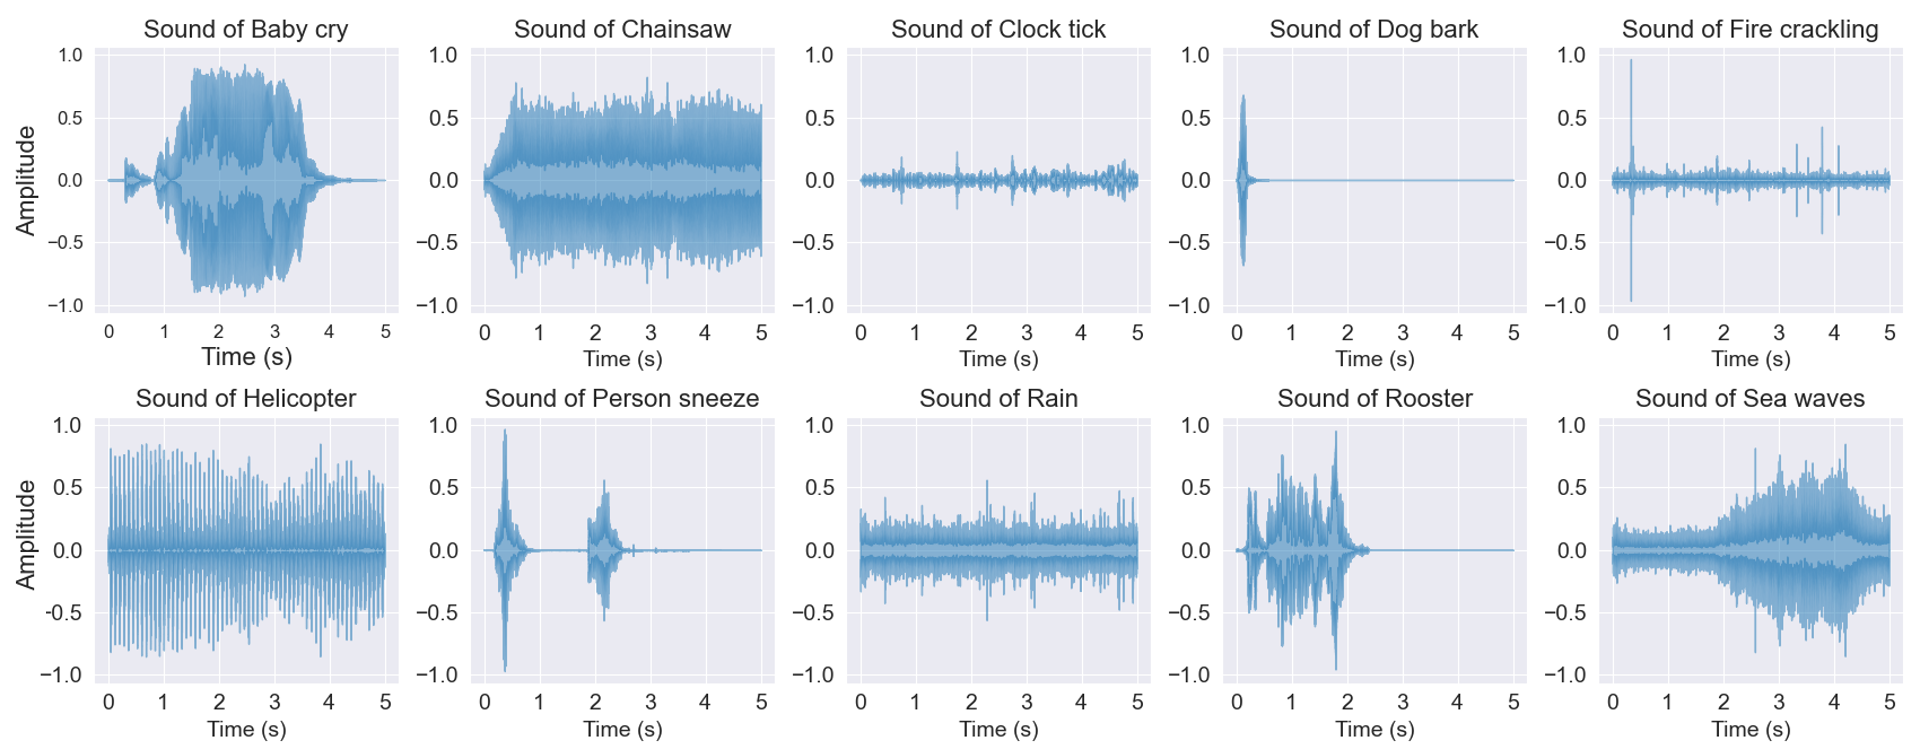
\includegraphics[width=1\textwidth]{resources/images/050-methods/Methods_dataset_ESC-10.png}
        \smallcaption{Source: Author}
        \label{fig:methods_dataset_ESC-10}
\end{figure}

The author proposed the extraction of two distinct types of features, precisely, \gls{zcr} and \gls{mfcc}, from each audio clip. The \gls{zcr} presents itself as a straightforward yet informative characteristic, while the application of \gls{mfcc} is widespread in the realm of speech processing and harmonic content analysis. The computation of \gls{mfcc}s was undertaken using the \index{Librosa}Librosa package \cite{McFee2015librosa_sw} with the default settings, giving rise to a frame length of 11.6 \gls{mi}\gls{s}. Following the exclusion of the 0\textsuperscript{th} coefficient, the initial 12 \gls{mfcc}s and the \gls{zcr} were combined for each clip via their respective mean and standard deviation across frames, resulting in a vector dimension of 26. These combined feature vectors were subsequently utilized as input for three distinct classifiers, namely, \gls{k-nn}, \gls{rf}, and \gls{svm} with a linear kernel. 

To assess the classifier performance, a 5-fold cross-validation regime was employed on the dataset ESC-10 during the learning phase, as the author made it explicitly in his dataset metadata the fold split from 1 to 5. Empirical evidence suggests that this particular number of folds provides test error rate estimates that effectively balance between avoiding excessively high bias and preventing high variance \cite{James2013}. For the \gls{k-nn}, the \index{hyperparameter}hyperparameter value for "k" was not specified in the article, however, in the code, it was defined as 8. The \gls{rf} ensemble consisted of multiple decision trees, where each tree was trained on a randomly selected subset of features and samples from the dataset, but the number of trees in the ensemble was not mentioned. Again, analyzing the code made it possible to see the author's decision for 500 estimators. For \gls{svm} with a linear kernel, no specific hyperparameters were mentioned either, but in the code, the regularization parameter C was set to 0.5 \cite{PiczakESC2015}.

The results showed that for the ESC-10 dataset: 
\begin{itemize}
    \item \gls{k-nn} achieved an average classification accuracy of 66.7\%;
    \item \gls{rf} ensemble achieved an average classification accuracy of 72.7\%;
    \item \gls{svm} had an average classification accuracy of 67.0\%. 
\end{itemize}

Considering the number of classes involved in this study, the ECS-10 presents itself as a better option to establish a baseline for the classifiers due to its compact size and its original purpose as proof of concept.

\subsection{BDLib2}
\label{subsec:dataset_BDLib2}

The BDLib2 Environmental Sound Dataset created by \textcite{Bountourakis2015} was designed to compare existing machine learning techniques for recognizing environmental sounds and determining the most effective one, focusing on analyzing discrete sound events rather than general acoustic environments, with the long-term goal of applying this knowledge to soundscapes recognition.

The dataset was constructed by identifying and extracting 10-second-long audio clips that represent distinct sound categories originally sourced from the BBC Complete Sound Effects Library \cite{BBC2023} and Freesound project \cite{Font_freesound2013}. The authors took utmost care during the clip selection process to ensure the absence of background noise and prevent any overlap between the sound categories.

All recordings in the dataset are uncompressed single channel files in WAV format, captured at a sampling rate of 44,100 \gls{hz} and analyzed with a precision of 16 bits, summing 180 labeled files, structured into 10 classes, namely (Figure \ref{fig:methods_dataset_BDLib2}):
\begin{itemize}
    \item Airplanes;
    \item Alarms;
    \item Applause;
    \item Birds;
    \item Dogs; 
    \item Motorcycles;
    \item Rain;
    \item Rivers;
    \item Sea waves;
    \item Thunders. 
\end{itemize}

\begin{figure}[htbp]
    \raggedright
        \caption{Waveform of random samples of each one of the classes within the dataset BDLib2.}
        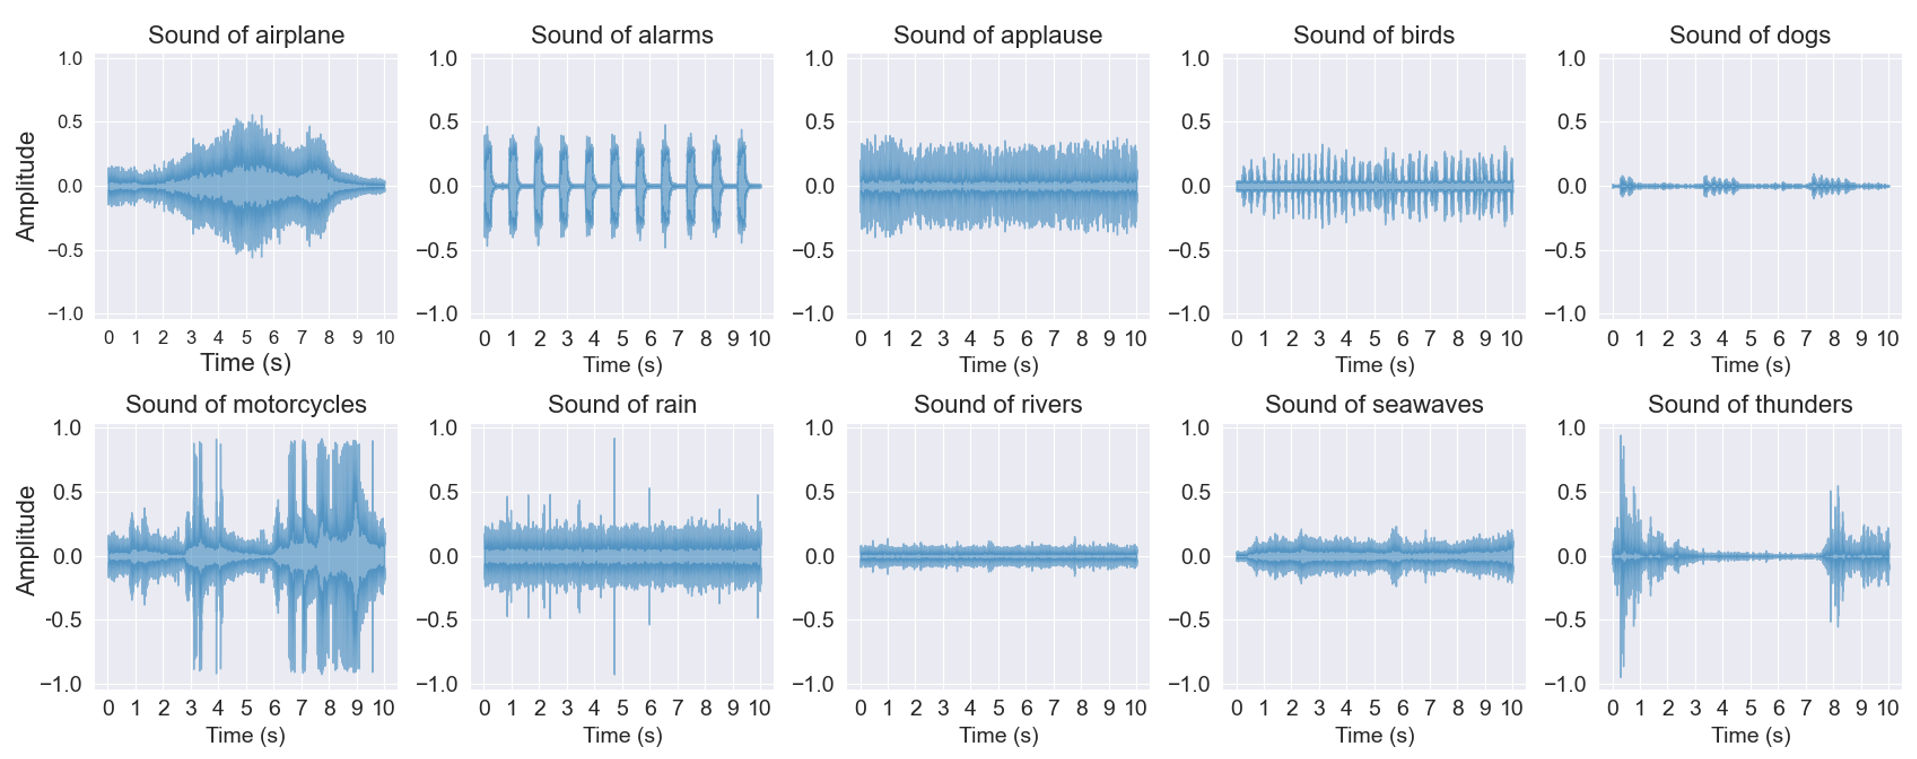
\includegraphics[width=1\textwidth]{resources/images/050-methods/Methods_dataset_BDLib2.png}
        \smallcaption{Source: Author}
        \label{fig:methods_dataset_BDLib2}
\end{figure}

While the original dataset experimental results \cite{Bountourakis2015} showed promising performance in classifying 7 different sound classes, it performed poorly in the recognition problem for 12 classes. Therefore, \textcite{Bountourakis2019} changed the library structure into new classes deliberately chosen to encompass a comprehensive range of sounds encountered in both indoor and outdoor soundscapes, aligning with established recognition schemes. To maintain diversity and authenticity, each class was uniformly represented in the database with 18 audio files, showcasing significant variations that reflect real-life scenarios.

Considering the total duration of the collected files amounts to 1,800 \gls{s}, which may be regarded relatively small for the intended classification task, two common data augmentation techniques were applied to address the problem of limited data, namely, time stretching with factors of 0.85 and 1.15, and pitch shifting by -4 and +4 semitones, carefully defined to ensure the semantic integrity of the transformed data. 

Following augmentation, the total duration of the complete database increased to 8,820 \gls{s}, which is comparable to the duration of similar reliable databases. It is worth noting that these augmentation techniques have been associated with improved model accuracy for environmental sound classification tasks \cite{Salamon2017} and are also presented in the systematic review of \textcite{Alli2022} for data augmentation and deep learning methods in sound classification.

In order to compare the frame-based method with temporal integration methods, several features shown in Table \ref{table:BDLib2_features_extracted} were extracted using two different window configurations: long windows for the frame-based method and short windows for the temporal integration methods. The short window had a duration of approximately 46 \gls{mi}\gls{s} with 50\% overlapping over 2,048 samples, while the long window had a duration of approximately 1.48 \gls{s} with 50\% overlapping over 65,536 samples. By extracting aggregated features over 64 subsequent short windows with 50\% overlapping, both methods achieved the same temporal resolution. For the sake of definition, 
texture window is commonly referred to as an early integration technique when the process is carried out at the feature extraction level by consolidating short-time features across a larger frame \cite{Bountourakis2019}.

\begin{table}[ht!]
    \caption[Features extracted in the BDLib2 dataset]{Extracted audio features, including their respective dimensions (with a default dimension of 1 when not explicitly stated) and their acronym.}
    \label{table:BDLib2_features_extracted}
    \centering
    \begin{tabular}{
        >{\centering\arraybackslash}m{0.67\textwidth} | >{\centering\arraybackslash}m{0.27\textwidth}}
        \Xhline{2\arrayrulewidth}
        \rowcolor{lightgray}
        \textbf{Feature} & \textbf{Symbol} \\
        \hline
        Zero Crossing Rate & ZCR \\
        Root Mean Square & RMS \\
        Relative Difference Function & RDF  \\
        Spectral Centroid  & CEN \\
        Spectral Spread & SPR\\
        Spectral Flux & FLU \\
        Root Mean Square & RMS \\
        Spectral Roll-Off & ROL \\
        Spectral Skewness & SKEW \\
        Spectral Kurtosis & KURT \\
        Spectral Entropy & ENTR \\
        Spectral Variability & VAR \\
        Spectral Smoothness & SMO \\
        Spectral Flatness Measure (24) & SFM \\
        Spectral Crest Factor (24) & CSF \\
        Brightness  & BRI \\
        Roughness & ROU \\
        Irregularity & IRR \\
        \gls{mfcc} (13) & \gls{mfcc} \\
        Delta \gls{mfcc} (13) & DMFCC \\
        \gls{lpcc} (12) & \gls{lpcc} \\
        \Xhline{2\arrayrulewidth}
    \end{tabular}
    \smallcaption{Source: \textcite{Bountourakis2019}, page 413}
\end{table}

 Besides the mean, \gls{std}, skewness, and kurtosis used in most temporal integration methods, 4 additional metrics were proposed:

 \begin{itemize}
    \item \gls{msd}: this metric quantifies the amount of variation and frequency of changes in successive feature values within a texture window;
    \item \gls{mcr}: inspired by \gls{zcr}, MCR estimates the alternations of successive feature values with respect to their mean value within a texture window;
    \item \gls{fla}: similar to Spectral Flatness, this metric calculates temporal flatness by dividing the geometric mean of feature values by their arithmetic mean within a texture window;
    \item \gls{crf}:  \gls{crf} is calculated by dividing the maximum value by the mean value of feature values within a texture window, similar to how it is used for waveforms.
\end{itemize}
	
To determine the most effective machine learning technique for the aforementioned dataset, 3 different methods for feature aggregation were proposed to generate feature vectors for sound classification, namely:

\begin{itemize}
    \item \gls{sfb}: a vector with a dimension of 100 considering all features extracted in Table \ref{table:BDLib2_features_extracted}, discarding the \gls{mfcc}-0 that is fundamentally related to the signal's energy;
    \item \gls{sti}: a vector with a dimension of 96 built through the mean, standard deviation, skewness, and kurtosis of the following 12 baseline features: \gls{mfcc}s, CEN, SPR, SKEW, KURT, ROL, ENTR, BRI, VAR, RMS, ZCR, and RDF;
    \item \gls{eti}: identical to \gls{sti} but including the 4 additional metrics previously described (MSD, MCR, FLA, and CRF), adding 96 dimensions to the vector leading to a final dimension of 192.
\end{itemize}

Feature ranking algorithms were employed to select the most relevant features for each method, followed by the utilization of \gls{lr}, \gls{ann}, and \gls{glm} classifiers for classification purposes. There was no mention of hyperparameters for \gls{lr} and \gls{glm}, on the other hand, the \gls{ann} architecture consisted of 2 hidden layers, with the number of neurons in each hidden layer being equivalent to half the sum of the input and output dimensions, and a dropout layer was then incorporated. The remaining parameters followed a conventional configuration: the \gls{relu} activation function was utilized for the intermediate layers, softmax function for the output layer, categorical cross-entropy was employed as the loss function, and Adam was utilized as the optimizer. The learning rate was set at 0.01 with a dropout rate of 25\%.

The training process involved splitting the sound files into a training set with 12 files per class and a testing set with 6 files per class, ensuring that the algorithms were tested on unseen data. To prevent overfitting and ensure unbiased results, a 3-fold cross-validation regime was employed during the learning phase following the dataset curator specifications (there are 3 distinct folds available after unzipping the downloaded files), nevertheless, it is noteworthy that such number of folds does not comply with the recommendations from \textcite{James2013}. The \gls{eti} method demonstrated higher accuracy than the \gls{sti} method, and among the classifiers, \gls{ann} performed the best with 81.5\% accuracy, followed by \gls{glm} with 80.4\% and \gls{lr} with 74.8\%. Nevertheless, in light of the objective of conducting comparisons with the other datasets in this study, it is more appropriate to utilize the findings from the \gls{sti}:

\begin{itemize}
    \item \gls{ann} achieved an average classification accuracy of  75.2\%;
    \item \gls{glm} following, with an average classification accuracy of 75.0\%;
    \item \gls{lr} by last, with an average classification accuracy of 73.6\%. 
\end{itemize}


\subsection{UrbanSound8K}
\label{subsec:dataset_US8K}

The authors of this dataset developed a taxonomy based on a subset of a previous taxonomy specific to urban acoustic environments, focusing on low-level sound sources like "car horn" and "jackhammer" instead of broader categories. They also analyzed noise complaints filed through New York City's 311 service to identify frequently complained about sound categories relevant to urban sound research \cite{Salamon2014}.

The UrbanSound dataset was created by downloading field recordings from the Freesound repository \cite{Font_freesound2013} and meticulously verifying each recording to ensure the presence of the sound of interest. After the filtering process, 1,302 recordings totaling over 27 hours of audio were obtained. In the next step, the recordings were labeled at the start and end times of every occurrence of a sound, and a salience description to indicate foreground or background perception was added. This resulted in 3,075 labeled occurrences, amounting to 18.5 hours of labeled audio. Finally, an additional subset called \gls{us8k} was created for sound source identification research, encompassing short audio snippets segmented into 4 \gls{s} slices using a sliding window approach with a 2 \gls{s} overlap, totaling 8,732 labeled files.

Using the open-source audio editing software \index{Audacity}Audacity, it was possible to identify that all recordings in the dataset are uncompressed multi-channel files (stereo) in WAV format, captured at a sampling rate between 8,000 and 192,000 \gls{hz} and analyzed with a precision of 32 bits, pre-arranged into ten folds (labeled fold1 to fold10) to facilitate the replication and comparison of the automatically generated classification results, namely (Figure \ref{fig:methods_dataset_US8K}):
\begin{itemize}
    \item air\_conditioner;
    \item car\_horn;
    \item children\_playing; 
    \item dog\_bark; 
    \item drilling; 
    \item engine\_idling; 
    \item gun\_shot; 
    \item jackhammer; 
    \item siren; 
    \item street\_music.
\end{itemize}

\vspace{12pt}

\begin{figure}[htbp]
    \raggedright
        \caption{Waveform of random samples of each one of the classes within the dataset \gls{us8k}.}
        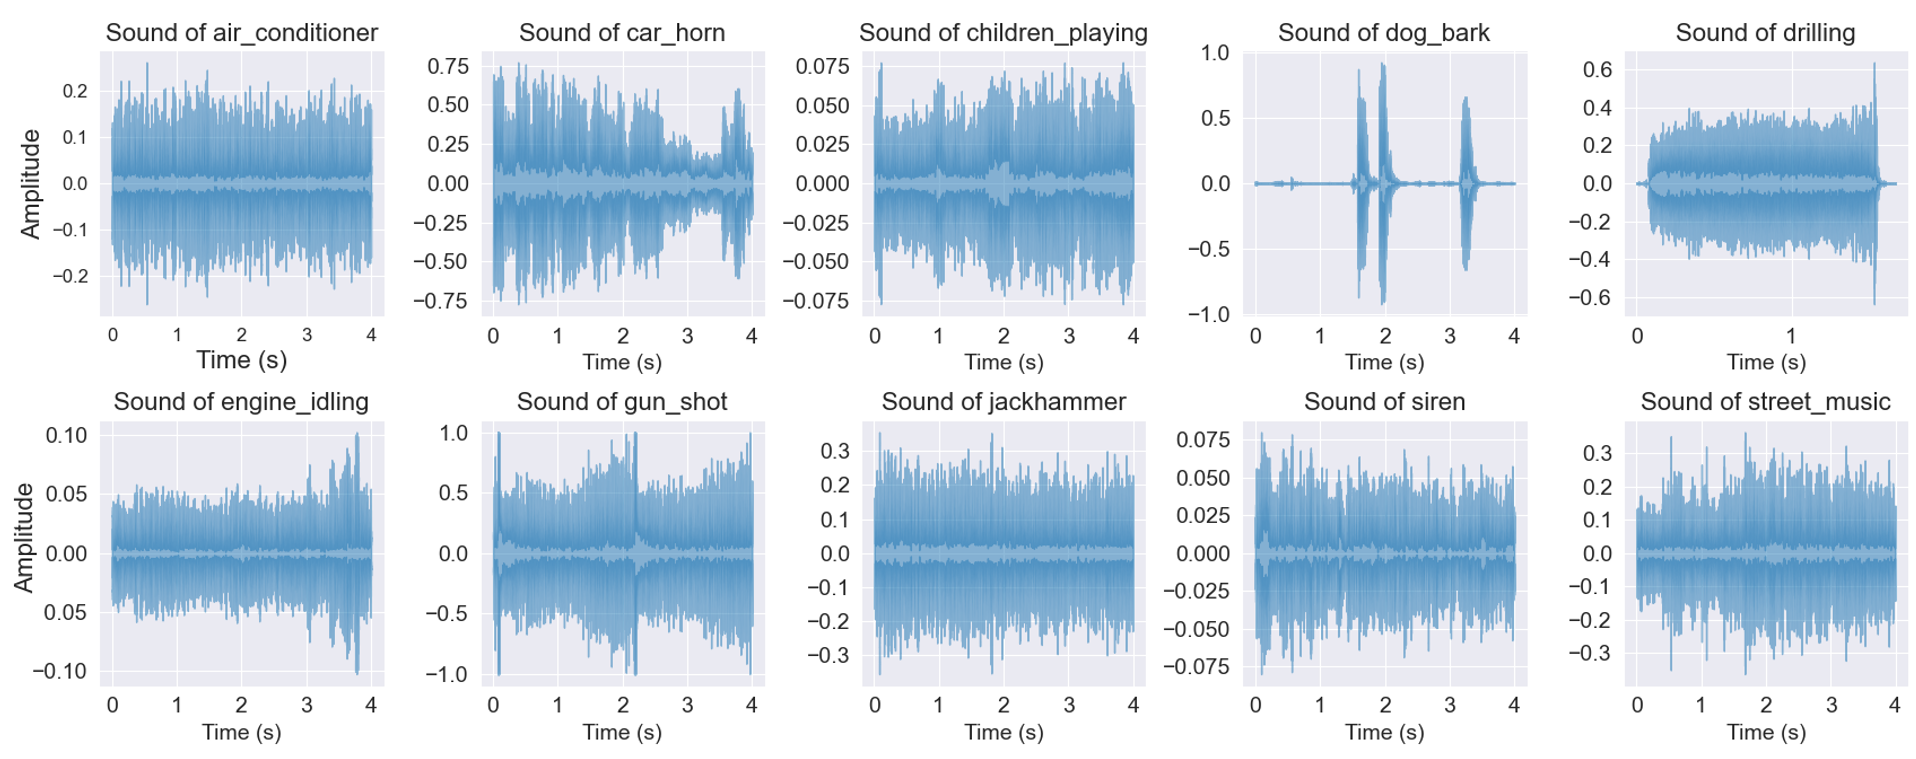
\includegraphics[width=1\textwidth]{resources/images/050-methods/Methods_dataset_US8K.png}
        \smallcaption{Source: Author}
        \label{fig:methods_dataset_US8K}
\end{figure}

The sound classification process was performed in the \gls{us8k}, aiming to learn about the characteristics of the dataset rather than an optimal combination of feature/classifier parameters. Considering the reasonable amount of recording hours in the dataset, the authors extracted \gls{mfcc} from the audio clips with no previous augmentation technique implemented. The features were extracted on a per-frame basis with a window size of 23.2 \gls{mi}\gls{s} and 50\% frame overlap using the first 25 \gls{mfcc} coefficients from the initially 40 Mel bands computed. Summary statistics such as minimum, maximum, median, mean, variance, skewness, and kurtosis along with mean and variance of first and second derivative coefficients were computed to create a feature vector of dimensionality equal to 225 per audio clip.

In order to experiment with different classification algorithms and audio clip lengths, 10-fold cross-validation was utilized through a random allocation process to ensure that clips from the same original recording were not used for both training and testing, thus avoiding artificially high classification accuracy results. The machine learning classifier considered were: Decision Tree, \gls{k-nn} with "k" set to 5 neighbors, \gls{rf} with 500 trees, \gls{svm} with an \gls{rbf} kernel, and a majority vote classifier named ZeroR. The authors analyzed the classifiers' performance considering a window of 1 \gls{s} to 10 \gls{s} for the audio clips, and most notably, it was noticed a uniform pattern in behavior across all classifiers, with performance maintaining stability from 10 \gls{s} to 6 \gls{s}, followed by a gradual decline. Yet, when focusing on the top-performing classifiers (\gls{svm} and \gls{rf}), the authors reported that there was no statistically significant distinction in performance between 6 \gls{s} clips and 4 \gls{s} clips, although the difference becomes significant when considering clips below 4 \gls{s}. As the dataset was published with a 4 \gls{s} window, the following results for each classifier were estimated below (values were not explicit, rather shown by a chart):

\begin{itemize}
    \item \gls{svm} was on top with an estimated classification accuracy of 69.0\%;
    \item \gls{rf} following, with an estimated classification accuracy of 66.0\%;
    \item \gls{k-nn} achieved estimated classification accuracy of 56.0\%;
    \item Decision Tree achieved an estimated classification accuracy of 48.0\%;
    \item Voting classifier by last, with an estimated classification accuracy of 10.0\%. 
\end{itemize}


\subsection{Tailored dataset (US8K\_AV)}
\label{subsec:dataset_US8K_AV}

The available datasets may not include the specific categories pertinent to the context outlined in this study, and generating new datasets is a labor-intensive and time-consuming task. To address this issue, the evaluation of existing datasets was conducted with consideration for the number of relevant classes that could potentially be integrated into the C-Bot during the third phase, as described in section \ref{sec:introduction_objective}. As illustrated in Figure \ref{fig:methods_dataset_US8K_AV}, the \gls{us8k} dataset includes four relevant classes relative to the study's objectives, whereas ESC-10 and BDLib2 contain only two. Moreover, \gls{us8k} offers more samples with greater diversity in terms of background and foreground mixtures. Consequently, a new dataset, named US8K\_AV (UrbanSound8K for Autonomous Vehicles), was developed using \gls{us8k} as the primary data source under specific conditions to optimize performance: irrelevant classes were eliminated, less relevant urban sounds were consolidated into a new class, and contextually relevant classes were preserved \cite{florentino2024}.

To maintain the same class distribution as the original dataset, the new class "background" was populated with 1,000 randomly selected samples from the original less relevant classes. Further on, the class "silence" was also added, sourced from the Freesound project \cite{Font_freesound2013} to complement the dataset, aiming to enhance the utility and accuracy of the inferences during live predictions. Special attention was given to preserving the dataset specification regarding the k-fold distribution, thus avoiding class contamination with sound segments from the same sound source. Upon completing this process, the US8K\_AV dataset comprised 4,908 files, distributed among 6 classes, preserving the 10-fold split for cross-validation, with a total duration of 4.94 hours of recorded sounds and 3.27 GB of total size. A detailed description of each of these classes is provided below, and the dataset statistics in Table \ref{table:US8K_AV_statistics}:

\begin{itemize}
    \item \textbf{"dog\_bark"}: characterized by a sharp and abrupt sound produced by canines, often indicating territorial defense or alertness to intrusions. Contains high variation in pitch and frequency over time. 0.87 h within 1,000 audio samples;
    \item \textbf{"children\_playing"}: this class encompasses a range of sounds, such as laughter, shouting, and running, typically generated by groups of children engaged in recreational activities in outdoor or indoor environments. 1.10 h within 1,000 audio samples;
    \item \textbf{"siren"}: mainly loud, high-pitched, oscillating tone used primarily by emergency vehicles such as ambulances, fire trucks, and police cars to signal their presence and urgency in traffic. 1.01 h within 929 audio samples;
    \item \textbf{"car\_horn"}: produced by motor vehicles, car horns generate a short, high-decibel honk intended to alert other drivers and pedestrians to potential hazards or to communicate driver intentions. 0.29 h within 429 audio samples;
    \item \textbf{"background"}: comprising a mixture of drilling, engine idling, jackhammer operations, and street music, this class represents ambient urban noise often encountered in metropolitan areas. The diverse soundscape serves as a backdrop that may mask or interfere with the detection of other distinct auditory events. 1.05 h within 1,000 audio samples;
    \item \textbf{"silence"}: characterized by a near-absence of discernible sound waves, this class represents periods of minimal or no auditory activity. Silence is essential for calibrating baseline noise levels and distinguishing between meaningful audio events and background noise. 0.61 h within 550 audio samples.
\end{itemize}


\begin{figure}[htbp]
    \raggedright
        \caption{Evaluation of the number of relevant classes within the datasets ESC-10, BDLib2, and \gls{us8k} related to autonomous vehicles and proposal for a tailored dataset based on the \gls{us8k} classes.}
        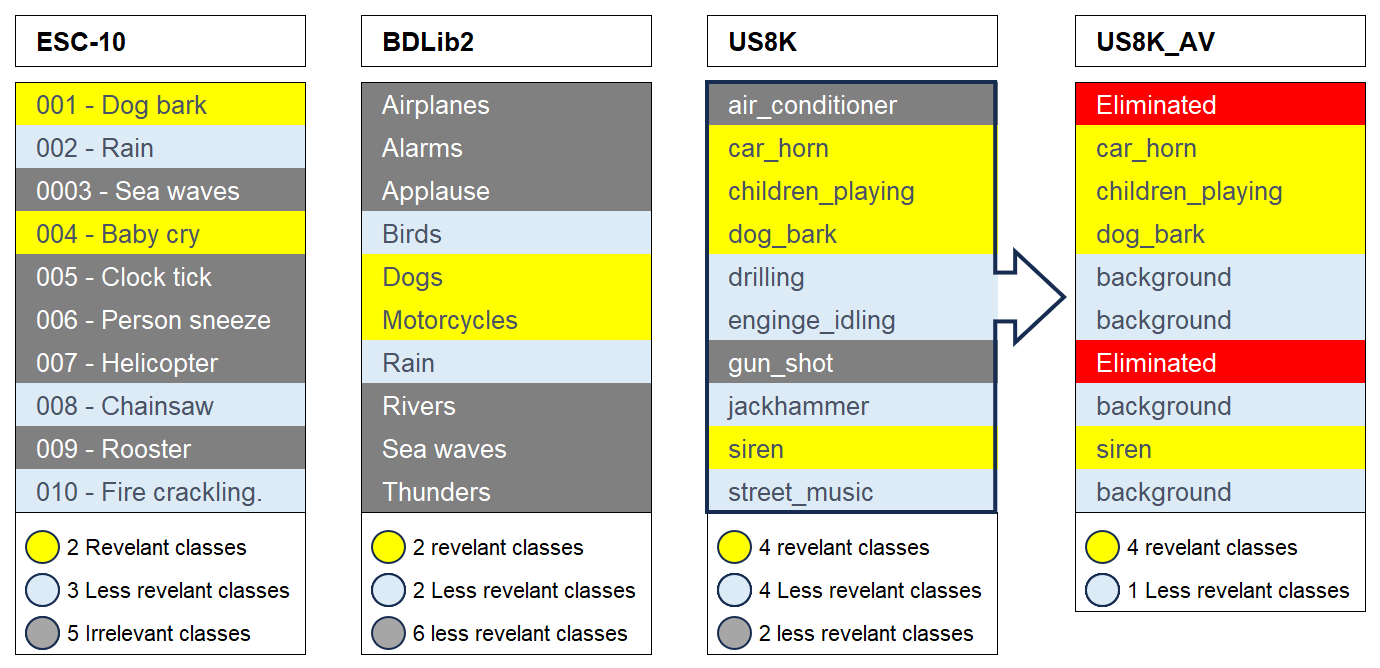
\includegraphics[width=1\textwidth]{resources/images/050-methods/Methods_dataset_US8K_AV.png}
        \smallcaption{Source: Author}
        \label{fig:methods_dataset_US8K_AV}
\end{figure}

\begin{table}[ht!]
    \caption[Statistics on the tailored dataset US8K\_AV]{Total size, number of files, unique sampling rates, and average duration corresponding to each class of the US8K\_AV dataset.}
    \label{table:US8K_AV_statistics}
    \centering
    \begin{tabular}{
        >{\arraybackslash}m{0.05\textwidth} | >
        {\raggedright\arraybackslash}m{0.15\textwidth} | >
        {\raggedright\arraybackslash}m{0.10\textwidth} | >
        {\raggedright\arraybackslash}m{0.11\textwidth} | >
        {\raggedright\arraybackslash}m{0.28\textwidth} | >
        {\raggedright\arraybackslash}m{0.13\textwidth}}
        \Xhline{2\arrayrulewidth}
        \rowcolor{lightgray}
        Fold & Folder name & Nr. files & Size & Min, Max sampling rates & Av. sample \\ 
        \rowcolor{lightgray}
        &  &  & (MB) & (Hz) & duration (s) \\        
        \hline
        1 & fold1 & 478 & 350.26 & 8,000 to 96,000 & 3.59 \\
        2 & fold2 & 485 & 334.86 & 11,025 to 96,000 & 3.58 \\
        3 & fold3 & 536 & 332.36 & 11,025 to 96,000 & 3.68 \\
        4 & fold4 & 599 & 422.08 & 11,025 to 96,000 & 3.63 \\
        5 & fold5 & 529 & 334.56 & 16,000 to 96,000 & 3.62 \\
        6 & fold6 & 460 & 276.28 & 11,025 to 96,000 & 3.62 \\
        7 & fold7 & 465 & 299.23 & 11,025 to 96,000 & 3.69 \\
        8 & fold8 & 441 & 279.12 & 8,000 to 192,000 & 3.58 \\
        9 & fold9 & 447 & 312.98 & 11,025 to 96,000 & 3.61 \\
        10 & fold10 & 468 & 328.68 & 11,025 to 96,000 & 3.62 \\
        \hline
    \end{tabular}
    \smallcaption{Source: Author}
\end{table}


\section{NORMALIZATION}
\label{sec:methods_normalization}

The concept of audio normalization entails the process of standardizing audio signals by harmonizing their amplitudes to a unified scale. Typically, this is achieved by manipulating the gain or volume of the audio while preserving its relative dynamics in order to establish a consistent level across all audio recordings, thereby minimizing the influence of factors such as disparate recording devices, microphone sensitivities, and environmental circumstances, bringing as consequences a consistency across different datasets, robustness to recording conditions and improved generalization \cite{Mueller2016}.

There are multiple audio normalization techniques, and the following compilation outlines the most pertinent approaches according to \textcite{Mueller2021}:

 \begin{itemize}
    \item Peak amplitude normalization: it involves adjusting the amplitude so that the highest point in the audio signal reaches a specified target level, ensuring that no part of the signal is clipped;
    \item \gls{rms} normalization: this method takes into account the overall energy distribution averaging its power signal and is less sensitive to short-term amplitude fluctuations;
    \item Perceptual loudness normalization: essentially identical to the \gls{rms} normalization but based on perceived loudness which considers human auditory perception.
    \item Frame-level normalization: it involves clipping the audio recording at a smaller time scale, such as individual frames or segments, to address variations within the audio signal over time, thus capturing dynamic patterns more effectively;
    \item Duration adjustment: while not strictly a normalization technique, adjusting the duration of audio segments to a common length is often performed in conjunction with amplitude normalization to ensure that the classifiers receive input of consistent duration in the training process.
\end{itemize}

Fundamentally, the authors of the aforementioned datasets stated they were already normalized to reach an amplitude peak of 80 \gls{db}, nonetheless, such statement was also confirmed during the data exploration in the Jupyter notebooks. \gls{rms} and perceptual loudness normalization were not explicitly mentioned in the related work, and though conceptually relevant, they were not utilized in this study.

During the preliminary classifiers experiments, the concept of frame-level normalization was investigated following the procedures of \textcite{Silva2019} and \textcite{Lhoest2021}. This involved dividing the audio signal into $n$ short audio clips, each lasting ~1 \gls{s} and overlapping with a 50\% margin (comprising 44 frames — around 46 \gls{mi}\gls{s} — at a sampling rate of 22,050 \gls{hz}, frame size of 1,024, and a hop length of 512). These shorter audio clips were only temporarily stored in an array until the relevant features were extracted from them. This technique was not considered in this study as an augmentation technique \textit{per se}, rather, it was used in section \ref{sec:methods_feature_extraction} as a supporting tool for one of the feature extraction methods.

Several classes in the datasets, particularly ESC-10, ESC-50, and BDLib2, contain audio files where the original sound constitutes only 30\% to 50\% of the total duration, with the remaining portion being silence, as illustrated in Figure \ref{fig:methods_normalization_original_wave_form}.

\begin{figure}[htbp]
    \raggedright
        \caption{Waveform of an audio sample from the dataset ESC-10, class "001 - Dog bark", file name: 3-170015-A.ogg, illustrating most of the audio duration as silence or near-silence.}
        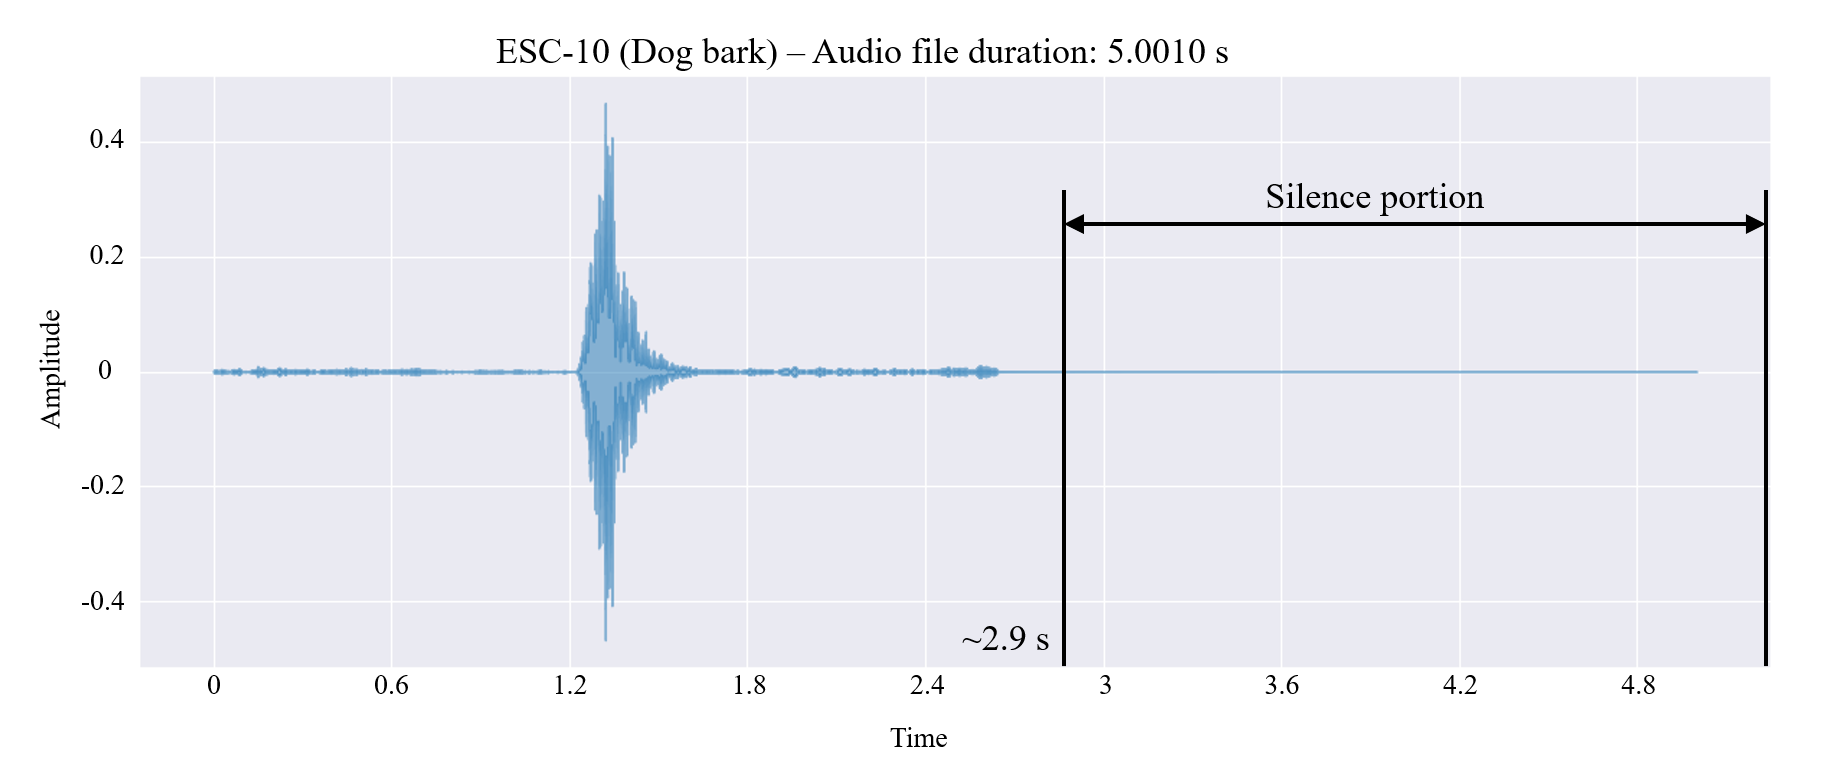
\includegraphics[width=1\textwidth]{resources/images/050-methods/Methods_normalization_original.png}
        \smallcaption{Source: Author}
        \label{fig:methods_normalization_original_wave_form}
\end{figure}

This type of audio data significantly reduces the accuracy of the classifiers, and therefore, the technique of duration adjustment was merged with trimming and implemented in this study. According to \textcite{Mushtaq2020b}, when applying the trim silence technique as a pre-processing method to the entire audio dataset, a common challenge arises in determining the precise threshold value in \gls{db} \underline{below the reference point} (80 \gls{db} confirmed by peak amplitude normalization), which indicates silence. The improper selection of this threshold value has the potential to lead to the loss of crucial information contained within the audio data, and although it stated in the article that the threshold of 40 \gls{db} has been settled as the most effective silence trimming value for the used datasets, this value was not suitable when merged with the duration adjustment technique as shown in Figure \ref{fig:methods_normalization_40_db_x_60_db_wave_form} where approximately 1.1 \gls{s} of the audio data was lost when compared with the threshold of this study.

\begin{figure}[htbp]
    \raggedright
        \caption{Waveform of the audio file 3-170015-A.ogg trimmed to 40 \gls{db} and 60 \gls{db}, resulting in approximately 1.1 \gls{s} of data loss.}
        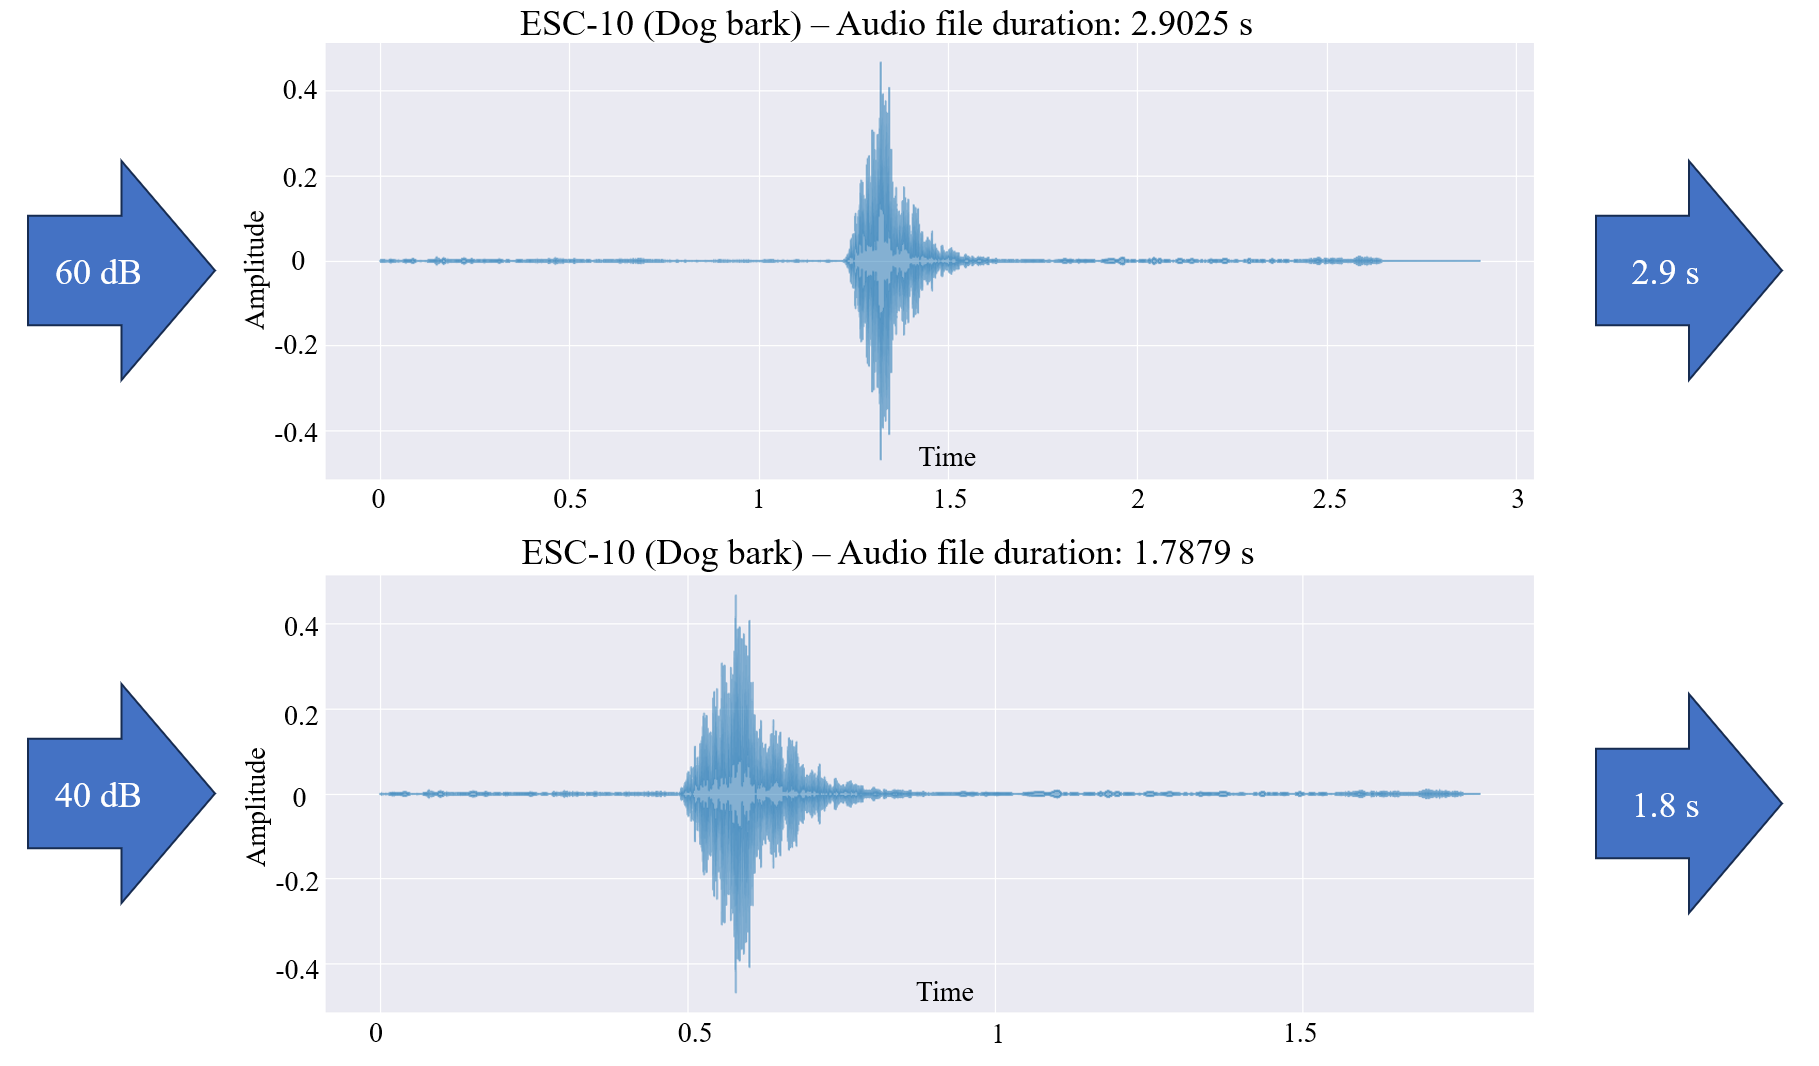
\includegraphics[width=1\textwidth]{resources/images/050-methods/Methods_normalization_comparison_40db_60db.png}
        \smallcaption{Source: Author}
        \label{fig:methods_normalization_40_db_x_60_db_wave_form}
\end{figure}


\begin{figure}[htbp]
    \raggedright
        \caption{Waveform of the audio file 3-170015-A.ogg trimmed to 60 \gls{db} and concatenated to reach the target duration of 5 \gls{s}.}
        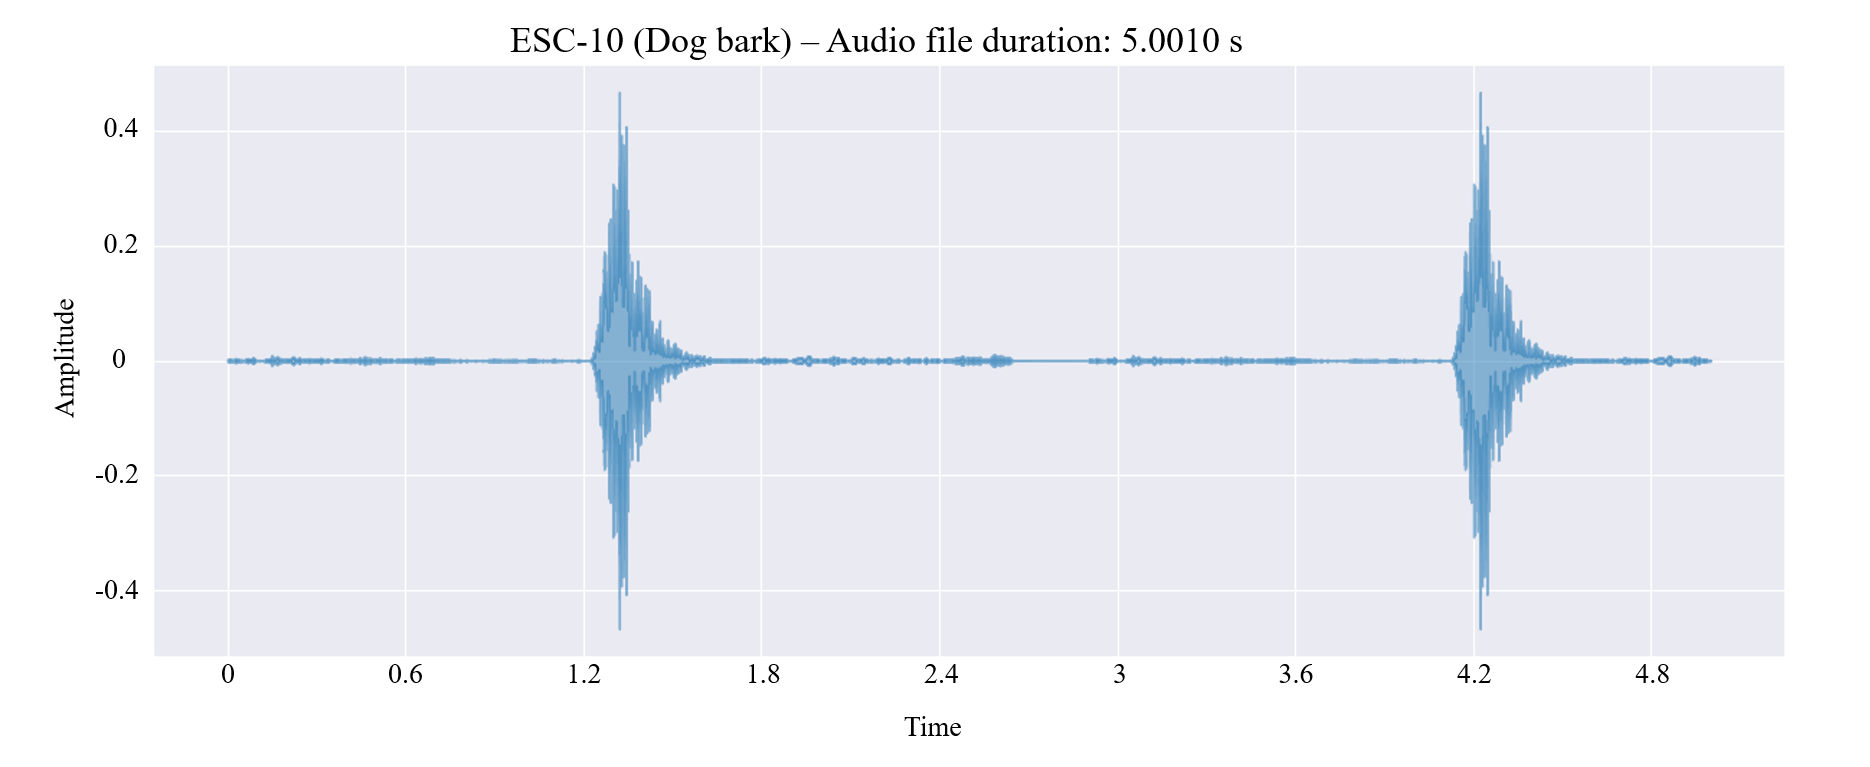
\includegraphics[width=1\textwidth]{resources/images/050-methods/Methods_normalization_normalized.png}
        \smallcaption{Source: Author}
        \label{fig:methods_normalization_normalized_audio_data}
\end{figure}

The value of 60 \gls{db} was settled as a threshold after several investigations using the split function of the package \index{Librosa}Librosa \cite{McFee2015librosa_sw}, which took an audio signal as input and returned a NumPy array of intervals, where each interval is represented as a tuple of start and end times (in samples) of non-silent audio. The for loop continues, concatenating the non-silent audio frames until the target duration is exactly achieved for each dataset (ESC-10: 5 \gls{s}, BDLib2: 10 \gls{s}, and UrbanSound8K: 4 \gls{s}). The final audio waveform of the normalized audio data is shown in Figure \ref{fig:methods_normalization_normalized_audio_data}. Significantly, the normalization process primarily focused on the duration adjustment rather than trimming in the datasets, as trimming was observed to occur infrequently (after the process, approximately 20\% of the audio data exhibited some form of trimming).


\section{AUGMENTATION}
\label{sec:methods_augmentation}

In general, augmentation techniques can help overcome the problem of limited labeled data, which is quite common in many application domains, and audio recognition is no exception. By artificially introducing variations in the audio data during training, audio augmentation expands the dataset and allows the models to learn more robust and discriminative features, thus improving their generalization capabilities, resulting in better-equipped models to handle real-world scenarios where the sounds may exhibit variations in pitch, duration, and amplitude. Additionally, audio augmentation helps the models become less sensitive to background noise by training them in a broader range of acoustic conditions.

In the systematic review of deep learning methods and data augmentation in sound classification, \textcite{Alli2022} ranked the technique of noise addition with the largest number of occurrences, accounting for 22 publications (39.2\%). The subsequent highest number of occurrences was attributed to the time shift method, encompassing 15 publications (26.7\%), following closely behind were the \gls{gan} based models and pitch shifting, each accounting for 12 publications (21.4\%). Additionally, alternative methods, namely, time stretching, mix-up, and background noise, summed 10 (17.8\%), 9 (16.1\%), and 8 (13.6\%) publications, respectively. 

 Time stretching, pitch shifting, dynamic range compression, and background noise were also used by \textcite{Salamon2017} in their deep convolutional neural network classifier. \textcite{Mushtaq2020b} utilized time stretching, pitch shifting, white noise addition, and silence trimming (that dwells between normalization and augmentation techniques) in their regularized deep convolutional neural network while \textcite{Bountourakis2019} considered only time stretching and pitch shifting. Techniques commonly used in the speech recognition helm, such as warping the features, masking blocks of frequency channels, and masking blocks of time steps \cite{Park2019}, were not found explicitly in the related work and, therefore, were not considered in this study.

After experimenting with the data augmentation within all the datasets, five techniques were selected and implemented in this study, namely, \textbf{time stretches quickly}, where the time of each audio clip of the dataset was stretched by a factor of 1.15, and \textbf{time stretch slowly}, acting in the opposite direction, the audio clip was slowed down by a factor of 0.85 (Figure \ref{fig:methods_augmentation_time_stretch}).

\begin{figure}[htbp]
    \raggedright
        \caption{Waveform of the audio file 3-170015-A.ogg augmented using the time stretch technique with factors 0.85 and 1.15.}
        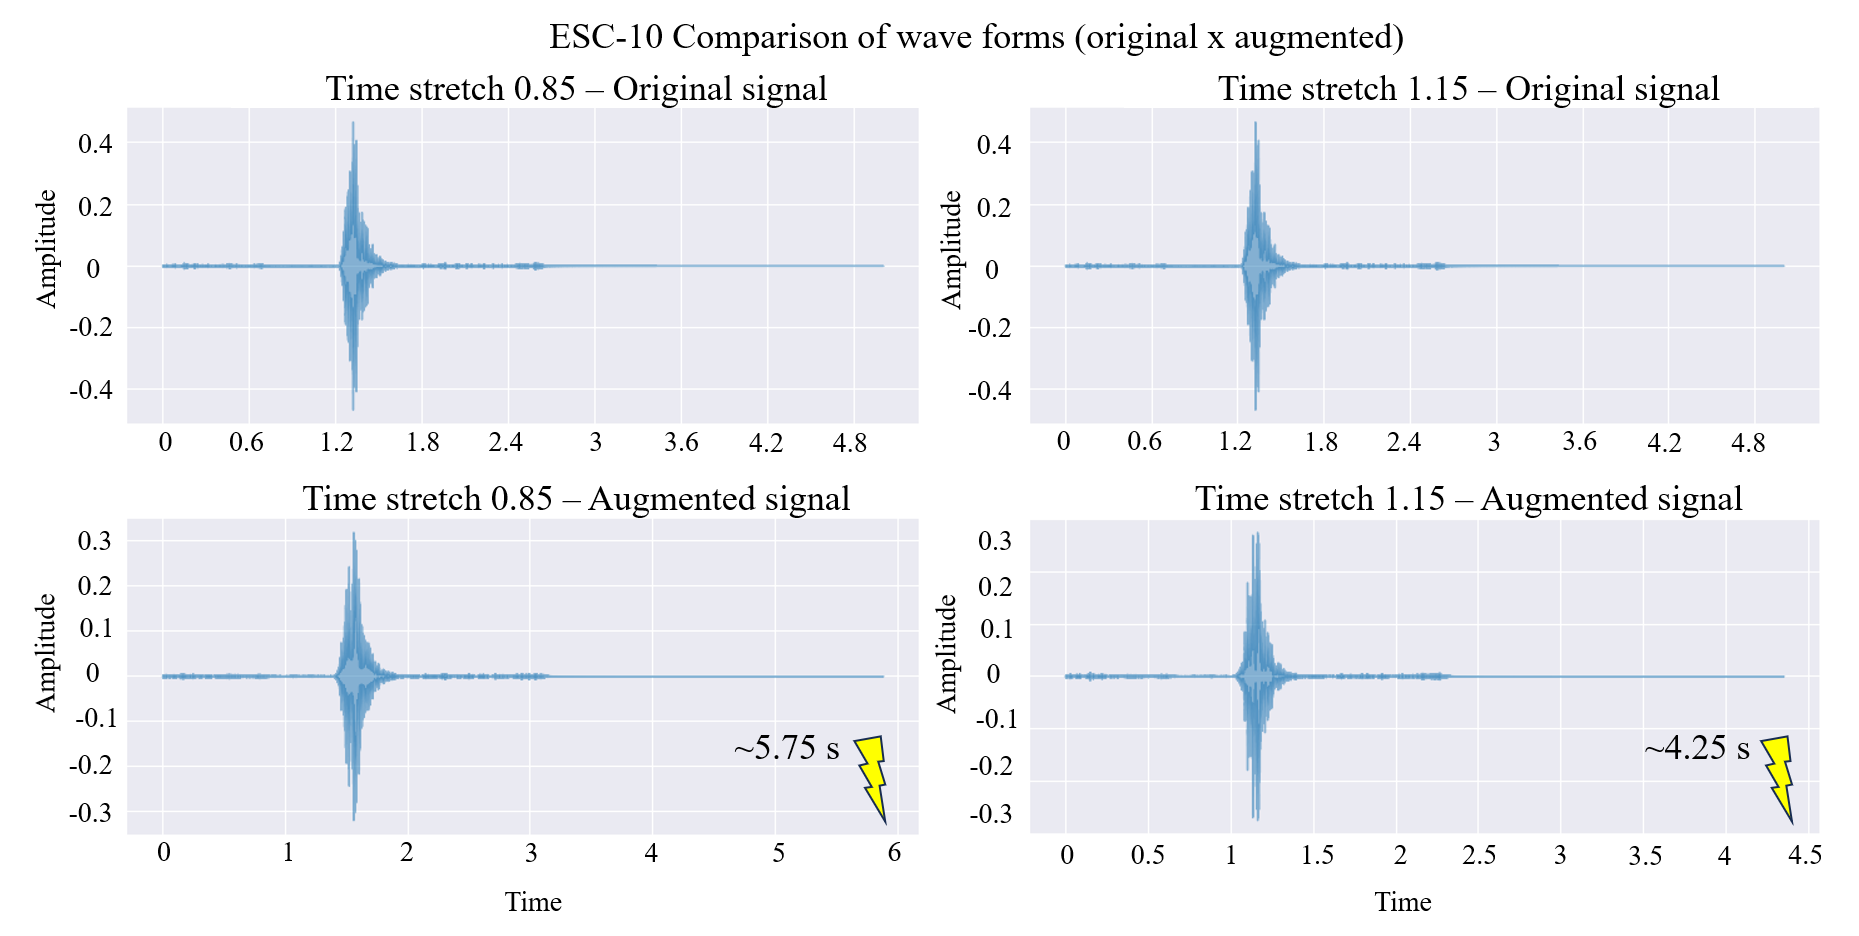
\includegraphics[width=.98\textwidth]{resources/images/050-methods/Methods_augmentation_time_stretching.png}
        \smallcaption{Source: Author}
        \label{fig:methods_augmentation_time_stretch}
\end{figure}

\textbf{Pitch shifting positively}, which increased the pitch of the audio clip in 4 semitones, and again, inversely, \textbf{pitch shifting negatively}, which decreased the pitch of the audio clip in 4 semitones, keeping the total duration of the audio file the same as shown in the spectrograms of Figure \ref{fig:methods_augmentation_pitch_shifting}. 

\begin{figure}[htbp]
    \raggedright
        \caption{Mel-frequency spectrogram of the audio file 3-170015-A.ogg augmented using the pitch shifting technique with +4 and -4 semitones.}
        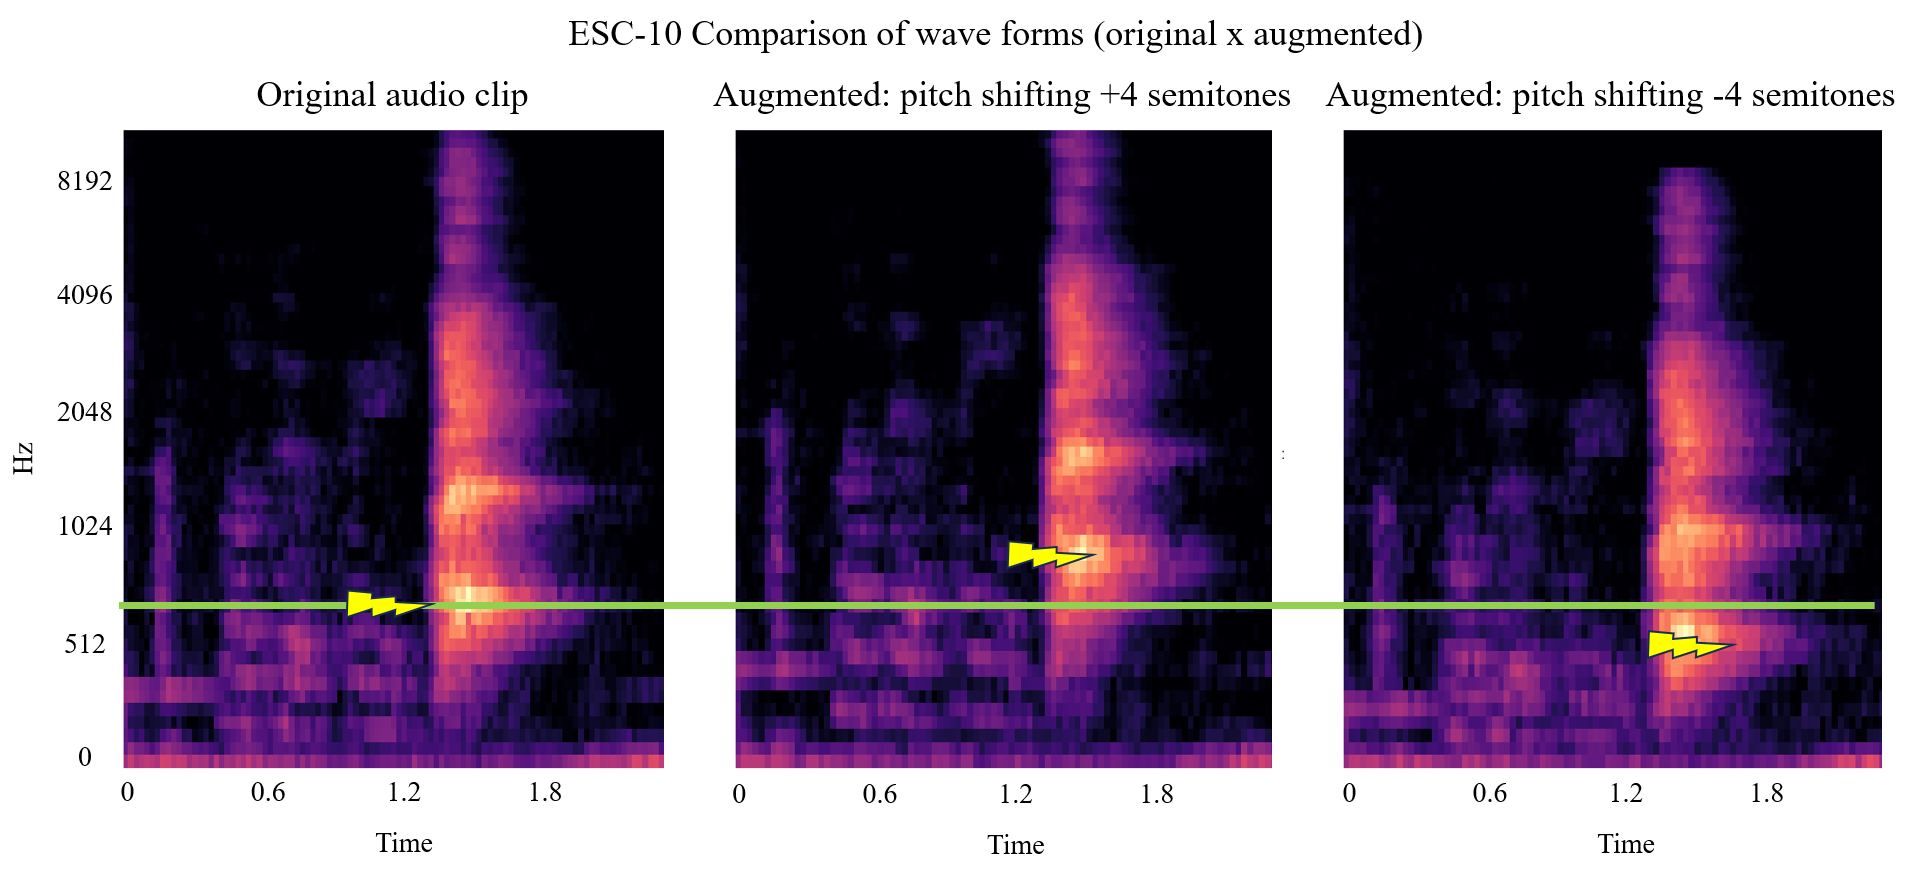
\includegraphics[width=.98\textwidth]{resources/images/050-methods/Methods_augmentation_pitch_shifting.png}
        \smallcaption{Source: Author}
        \label{fig:methods_augmentation_pitch_shifting}
\end{figure}

And finally, \textbf{time shifting randomly}, where the algorithm initializes a random integer (start\_) within the range [-4,800, 4,800] using NumPy random.uniform. Depending on the value of start\_, a time shift is applied to the audio clip. If the start\_ is negative, the audio is shifted to the right by start\_ samples, and random noise is added at the beginning. If the start\_ is positive, the audio is shifted to the left by start\_ samples and random noise is added at the end (Figure \ref{fig:methods_augmentation_time_shifting}).

\begin{figure}[htbp]
    \raggedright
        \caption{Waveform of the audio file 3-170015-A.ogg augmented using the time shifting technique when start\_ was initialized with +4,800 and random noise was added in the end.}
        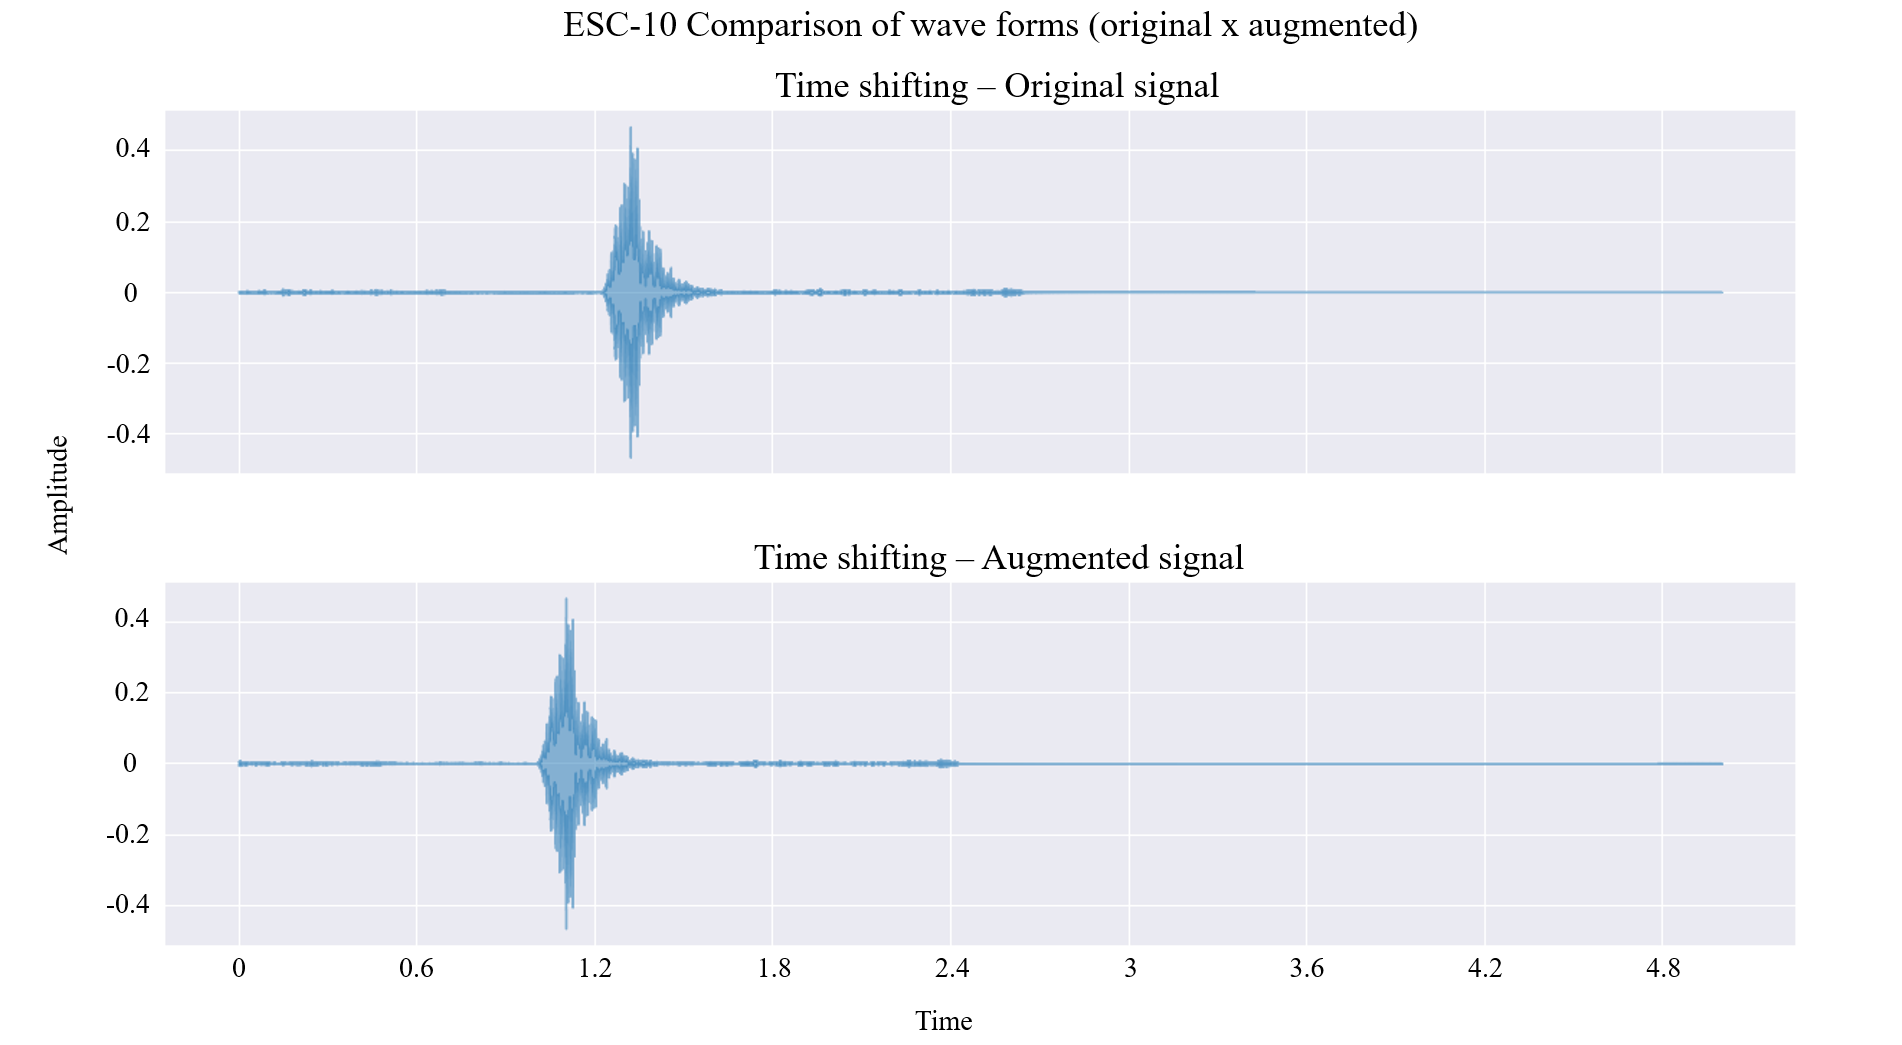
\includegraphics[width=1\textwidth]{resources/images/050-methods/Methods_augmentation_time_shifting.png}
        \smallcaption{Source: Author}
        \label{fig:methods_augmentation_time_shifting}
\end{figure}

After the implementation of the five augmentation techniques, the dataset characteristics were changed, as described in Table \ref{table:summary_datasets_before_and_after_augmentation}, comparing the values before and after the process.

\begin{table}[ht!]
    \caption[Comparison between the original datasets and their augmented versions]{Characteristics of the datasets before and after the implementation of the augmentation process, including the total size of the compiled features file in format .PKL (Python library Pickle).}
    \label{table:summary_datasets_before_and_after_augmentation}
    \centering
    \begin{tabular}{p{2.7cm}|p{1.6cm}|p{1.7cm}|p{1.7cm}|p{1.6cm}|p{1.7cm}|p{1.7cm}}
        \Xhline{2\arrayrulewidth} 
        \rowcolor{lightgray}
        \textbf{Dataset} & \hfil\textbf{Samples} & \hfil\textbf{Duration} & \hfil\textbf{Features} & \hfil\textbf{Samples} & \hfil\textbf{Duration} & \hfil\textbf{Features}\\
        \rowcolor{lightgray}
          & \hfil (units) & \hfil (h) & \hfil (\gls{m}\gls{b}) & \hfil(units) & \hfil(h) & \hfil(MB)\\    
        \Xhline{2\arrayrulewidth}
        \rowcolor{gray!20} & \multicolumn{3}{c|}{\textbf{Before Augmentation}} & \multicolumn{3}{c}{\textbf{After Augmentation}} \\
        \hline
        ESC-10 & \hfil 400 & \hfil 0.55 & \hfil 2.2 & \hfil 2,400 & \hfil 3.33 & \hfil 1,213\\
        BDLib2 & \hfil 180 & \hfil 0.50 & \hfil 155.6 & \hfil 1,080 & \hfil 3.00 & \hfil 1,088\\
        UrbanSound8K & \hfil 8,732 & \hfil 8.75 & \hfil 3,034 & \hfil 52,392 & \hfil 52.20 & \hfil 21,215\\
        \Xhline{2\arrayrulewidth}
    \end{tabular}
    \smallcaption{Source: Author}
\end{table}


\section{FEATURE EXTRACTION}
\label{sec:methods_feature_extraction}

There is a wide range of audio features that can be broadly categorized into perceptual and physical features based on their semantic interpretation, as described in section \ref{subsec:audio_fundamentals_audio_features}. Perceptual features, such as pitch, loudness, rhythm, and timbre, approximate properties that are perceived by human listeners. Conversely, physical features describe audio signals in terms of mathematical, statistical, and physical properties and are further classified as temporal features and spectral features based on the representation domain \cite{Lhoest2021}. Classical machine learning classifiers typically require the extraction of diverse features from the raw audio signal. While it is possible to input raw audio into classifiers based on CNN models, such classifiers tend to have numerous layers and a substantial number of parameters. This is because CNN models must learn to extract features from the raw audio in the early layers of its architecture \cite{Chu2023}.

This section introduces the physical features and their extraction process utilized during the implementation of the experiments, initially using "feature engineering" and then "aggregated features" for the \gls{cnn} 2D classifiers. The method of selecting features tailored to specific classification tasks is referred to in the literature as feature engineering. All of the hereafter audio features are extracted using \index{Librosa}Librosa \cite{McFee2015librosa_sw} due to its variety of tools for feature extraction, easy-to-use implementation, support for ARM-based processors, and seamless integration with the Python library \index{scikit-learn}scikit-learn \cite{scikitle61}.

Once the audio features have been thoughtfully selected, these "handcrafted features" formatted into a features array can be used in both machine learning and neural network classifiers instead of the raw audio, allowing the utilization of a smaller model that is more suitable for embedded devices.

For comparison purposes, the feature extraction process of the audio files in the datasets was divided into two methods. The first method (Figure \ref{fig:methods_feature_extraction_leap_window}) employed a sliding or leap window, following the procedures described by \textcite{Silva2019} and \textcite{Lhoest2021} in section \ref{sec:methods_normalization}, as a normalization technique (frame-level normalization). The choice of a sampling rate of 22,050 \gls{hz} was based on the work of \textcite{Salamon2017}, and although \textcite{PiczakESC2015} and \textcite{Bountourakis2015} utilized a sampling rate of 44,100 \gls{hz}, preliminary experiments showed no significant benefits of using a higher sampling rate, and the downturn of such choice was a larger compiled features file that ultimately consumed more memory allocation and longer training time. The selection around 1 \gls{s} leap window with 50\% overlap was based on the fact that the sounds within the datasets, while non-stationary, did not exhibit abrupt changes over time. Larger leap window sizes, although slightly beneficial in terms of accuracy \cite{Salamon2017}, were not considered. 

\begin{figure}[htbp]
    \raggedright
        \caption{Frame level normalization and feature extraction for a sample of the dataset ESC-10 (5 \gls{s} duration, with 9 windows and 44 frames on each window).}
        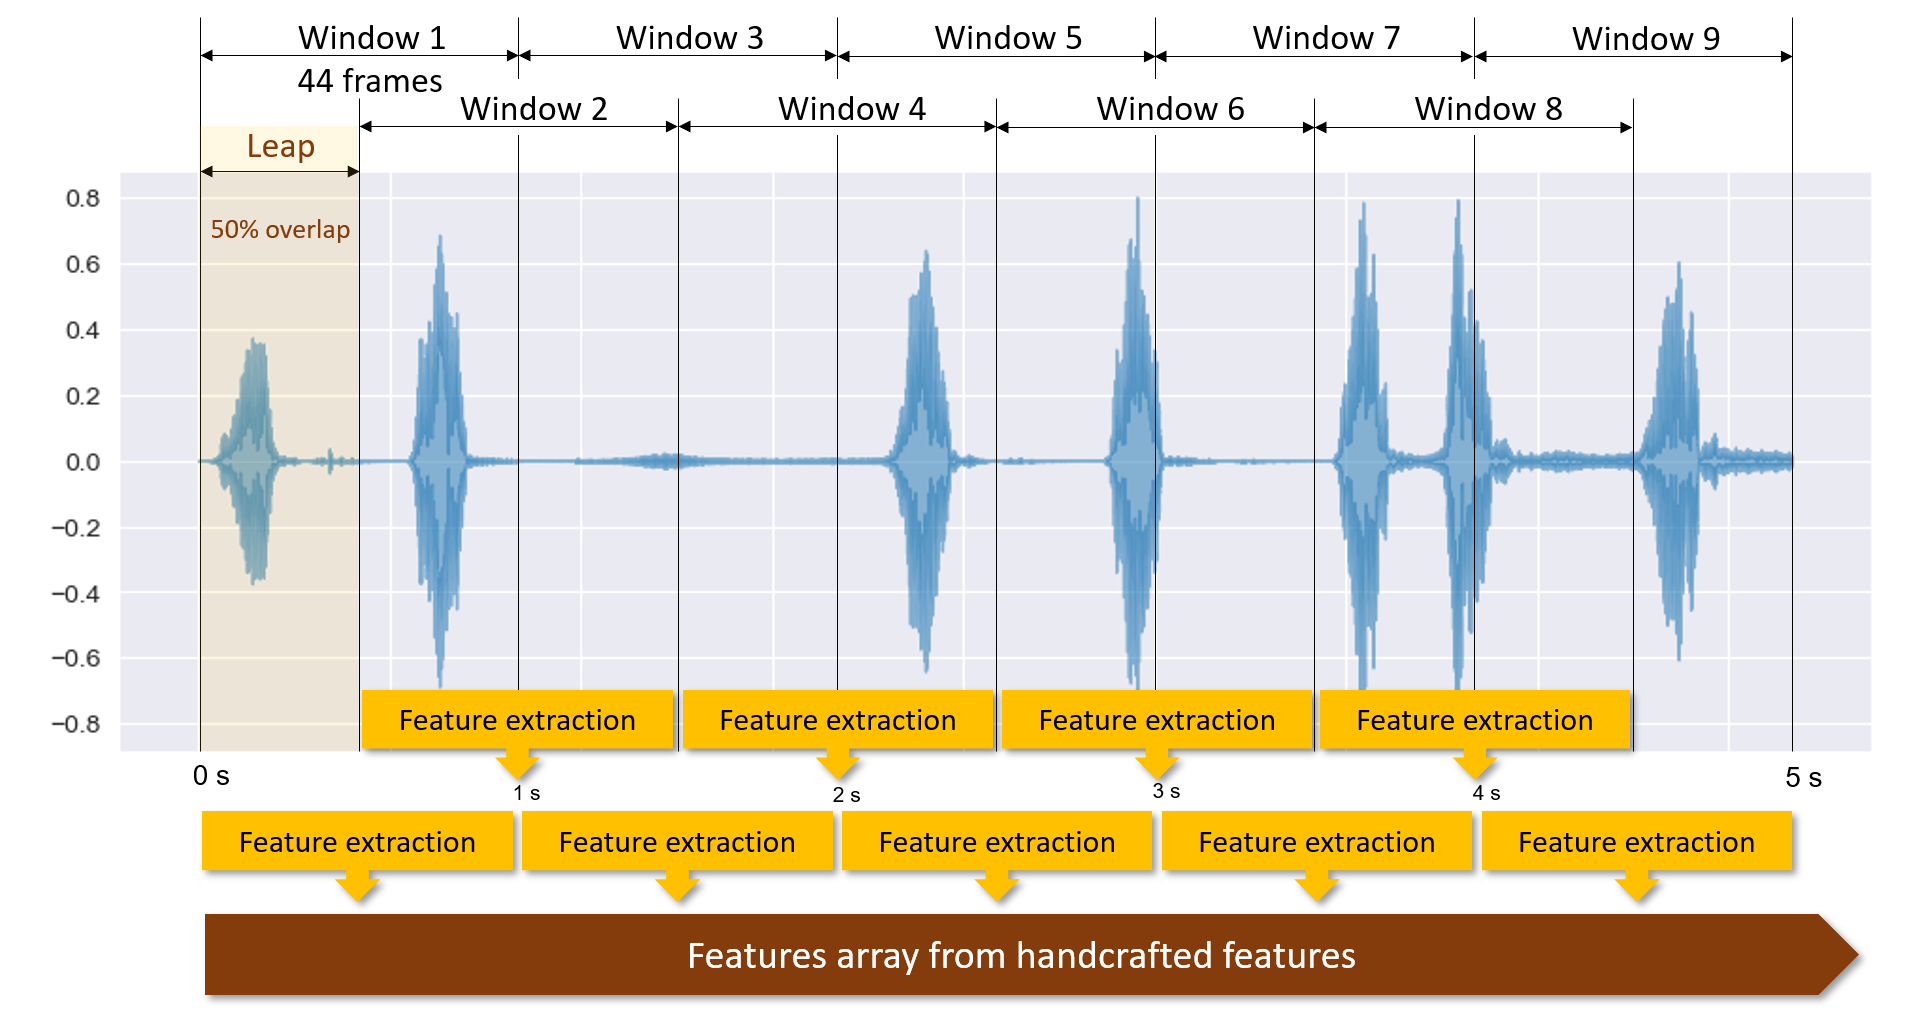
\includegraphics[width=1\textwidth]{resources/images/050-methods/Methods_feature_extraction_1_BDLib2.png}
        \smallcaption{Source: Author}
        \label{fig:methods_feature_extraction_leap_window}
\end{figure}

The second method involved using the entire audio file (single window) as input for the feature extraction process (Figure \ref{fig:methods_feature_extraction_single_window}), as proposed by the authors of the datasets ESC-10 \cite{PiczakESC2015}, BDLib2 \cite{Bountourakis2015}, and UrbanSound8K \cite{Salamon2017}, but for normalization purposes, utilized the same sampling rate of 22,050 \gls{hz} as the first method. \Textcite{Vandendriessche2021} also utilized the same technique in their \gls{cnn} classifier embedded in \gls{fpga}s and \gls{tpu}s.


\begin{figure}[htbp]
    \raggedright
        \caption{Single window or complete audio feature extraction for a sample of the dataset ESC-10 (5 \gls{s} duration, with 1 window and 216 frames).}
        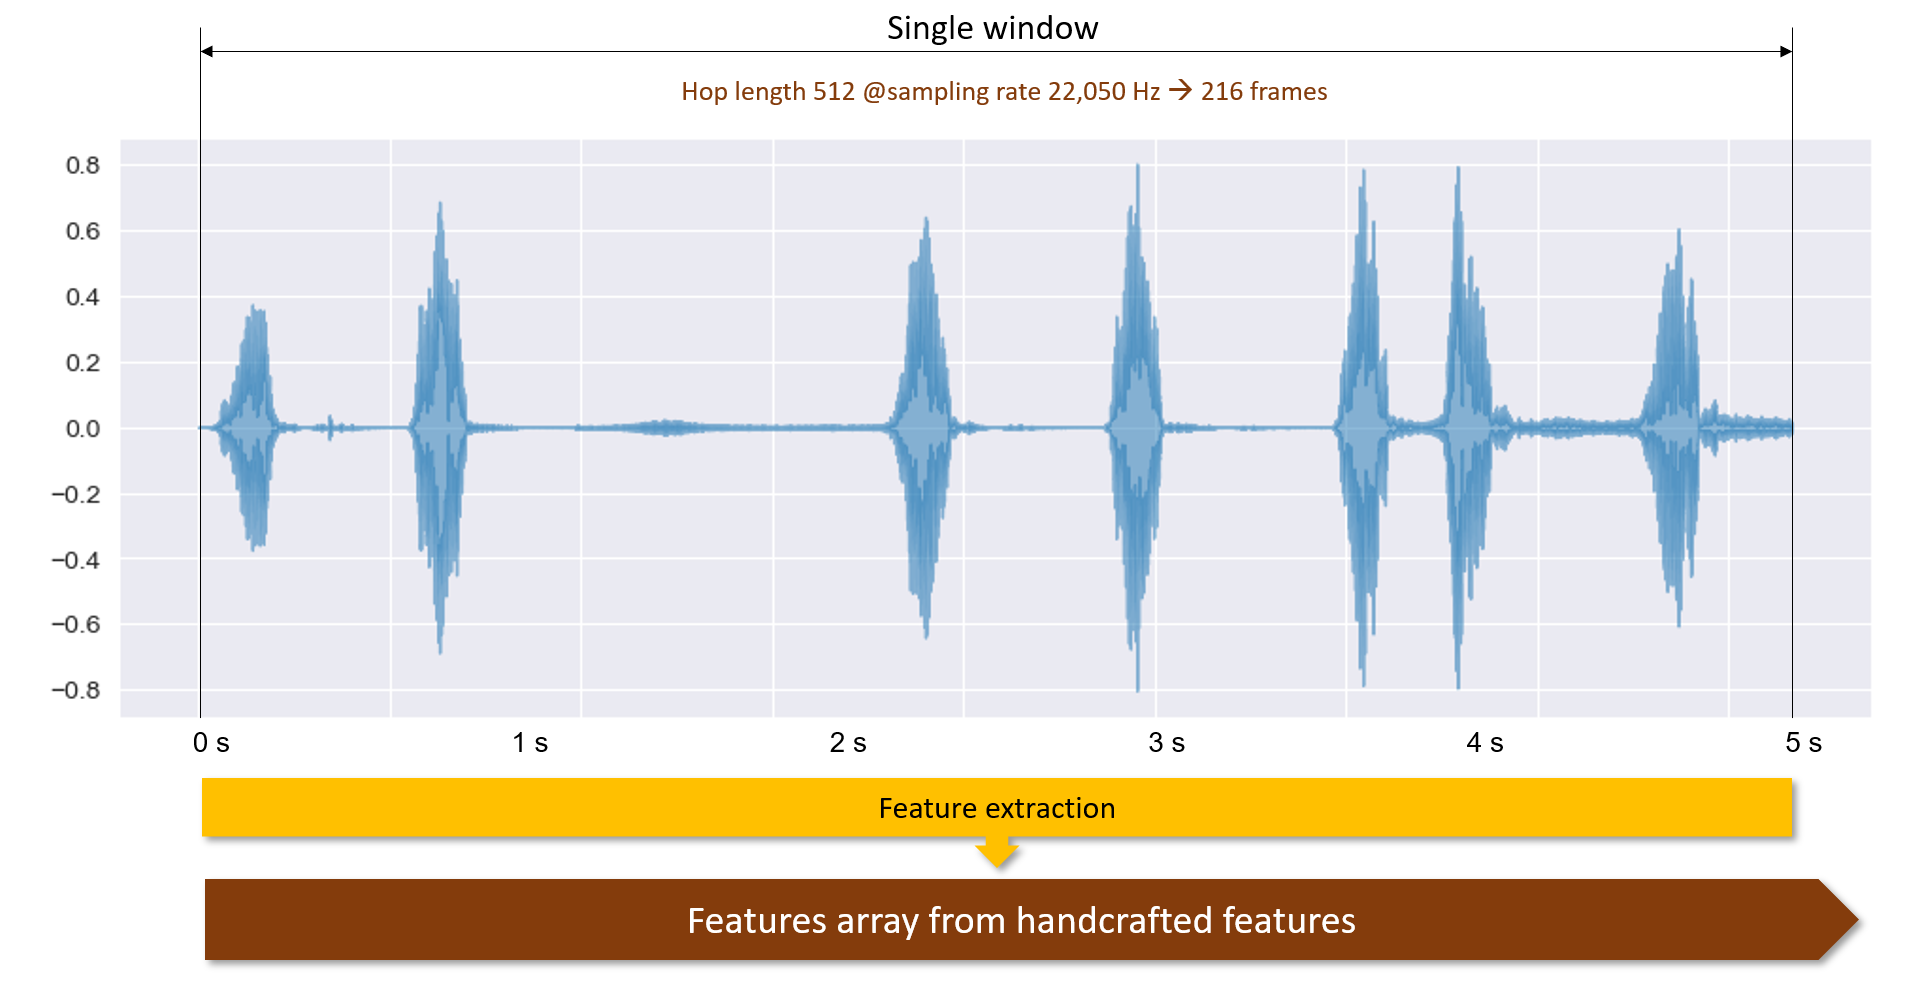
\includegraphics[width=1\textwidth]{resources/images/050-methods/Methods_feature_extraction_2_BDLib2.png}
        \smallcaption{Source: Author}
        \label{fig:methods_feature_extraction_single_window}
\end{figure}

The features selected were defined in section \ref{subsec:audio_fundamentals_audio_features}, and the feature extraction process utilized a Hann window \cite{Blackmann1958} with a hop length of 512, sampling rate of 22,050 \gls{hz} and frame size of 1,024 (around 46 ms) for \gls{rms} and \gls{zcr} to achieve a higher time resolution, and $n\_fft$ (number of frames for the \gls{stft}) of 2,048 for the remaining features to increase the frequency resolution. The number of Mel was 128, and \gls{mfcc} was 13.

In the first method, since the number of frames and hop length is fixed, resulting in a window of 1 \gls{s} with 50\% overlapping, the number of windows for the feature extraction on each dataset is calculated by $N_w = audioduration * 2 -1$, leading to 9 windows for the ESC-10, 19 windows for the BDLib2 and 7 windows for the \gls{us8k}.

In both methods, the features with only one coefficient had their per-frame values calculated by mean, on the other hand, the features containing more than one coefficient, had their per-frame values for each coefficient summarized across time using statistics, namely, mean, median, \gls{std}, skewness and kurtosis. The exceptions were Mel with only mean, Delta \gls{mfcc}, and Delta-Delta \gls{mfcc} with mean and \gls{std} calculated.  The result was an array containing 375 features, as shown in Table \ref{table:features_array_composition}.

\begin{table}[ht!]
    \caption[Composition of the first features array]{Composition of the features array utilized in the machine learning, \gls{ann}, and \gls{cnn} 1D classifiers after the feature extraction process.}
    \label{table:features_array_composition}
    \centering
    \begin{tabular}{p{3cm}|p{2.5cm}|p{1.2cm}|p{1.9cm}|p{3.5cm}|p{1.3cm}}
        \Xhline{2\arrayrulewidth} 
        \rowcolor{lightgray}
        \textbf{Feature} & \hfil\textbf{Coefficients} & \hfil\textbf{Mean} & \hfil\textbf{Mean, \gls{std}} & \textbf{Mean, \gls{std}, median, skewness, kurtosis} & \hfil\textbf{$\sum{}$}\\
        \Xhline{2\arrayrulewidth}
        \gls{rms} & \hfil 1 & \hfil 1 & \hfil --- & \hfil --- & \hfil 1 \\
        \gls{zcr} & \hfil 1 & \hfil 1 & \hfil --- & \hfil --- & \hfil 1 \\
        \gls{sc} & \hfil 1 & \hfil 1 & \hfil --- & \hfil --- & \hfil 1 \\
        \gls{sb} & \hfil 1 & \hfil 1 & \hfil --- & \hfil --- & \hfil 1 \\
        \gls{srp} & \hfil 1 & \hfil 1 & \hfil --- & \hfil --- & \hfil 1 \\
        Mel & \hfil 128 & \hfil 1 & \hfil --- & \hfil --- & \hfil 128 \\
        $\triangle$ \gls{mfcc} & \hfil 13 & \hfil --- & \hfil 2 & \hfil --- & \hfil 26 \\
        $\triangle\triangle$ \gls{mfcc} & \hfil 13 & \hfil --- & \hfil 2 & \hfil --- & \hfil 26 \\
        \gls{mfcc} & \hfil 13 & \hfil --- & \hfil --- & \hfil 5 & \hfil 65 \\
        \gls{sct} & \hfil 7 & \hfil --- & \hfil --- & \hfil 5 & \hfil 35 \\
        Chroma & \hfil 12 & \hfil --- & \hfil --- & \hfil 5 & \hfil 60 \\
        Tonnetz & \hfil 6 & \hfil --- & \hfil --- & \hfil 5 & \hfil 30 \\
        \hline       
        \rowcolor{gray!20} 
        \textbf{Total} & \multicolumn{4}{c|}{} & \hfil\textbf{375} \\
        \Xhline{2\arrayrulewidth}
    \end{tabular}
    \smallcaption{Source: Author}
\end{table}


Finally, a dedicated algorithm was implemented to extract spectral features from the image domain formatting them into "aggregated features" for the \gls{cnn} 2D model. This approach leverages the well-documented strengths of convolutional neural networks in two-dimensional image classification tasks by utilizing a pseudo-image format based on log-mel-spectrograms aggregated with their first and second derivatives, known as Delta and Delta-Delta, respectively. The log-mel-spectrogram provides a visual representation of an audio signal's frequency content over time, computed using \gls{stft} and triangular filters. In this representation, the frequency axis (Y-axis) is scaled according to the Mel scale, which approximates human auditory perception \cite{Moore2013}, while the amplitude values are converted to a logarithmic scale. The shape of the pseudo-image is contingent upon the audio duration, represented by the number of frames containing the audio samples. For the sliding window method, the number of frames (X-axis) is fixed at 44 frames (equivalent to 1 \gls{s} of audio). For the single window method, it varies according to the audio duration: 173 frames for \gls{us8k} and US8K\_AV (4 \gls{s}), 216 frames for ESC-10 (5 \gls{s}), and 413 frames for BDLib2 (10 \gls{s}). In both methods, the number of Mel bands was set to 60, resulting in log-mel-spectrogram dimensions of 60 x 173, 60 x 216, and 60 x 431, respectively. For the sliding window method, the dimension remains consistent at 60 x 44 across all datasets.

The first and second derivatives are computed to capture temporal dynamics and spectral acceleration changes, while retaining identical dimensions as the original log-mel-spectrogram. These three arrays are subsequently stacked along the frequency band axis, producing a composite array with dimensions of 180 x 44 when considering the sliding window method, as depicted in Figure \ref{fig:methods_feature_extraction_log-mel_spectrogram}. By feeding this pseudo-image into the \gls{cnn} 2D model, the resultant feature map encapsulates both static spectral properties and dynamic temporal variations, thereby enhancing the discriminative power of this classifier.

\begin{figure}[htbp]
    \raggedright
        \caption{Log-mel-spectrogram aggregated with first and second derivatives for a sample of the dataset US8K (sliding window with 1 \gls{s} duration and 44 frames).}
        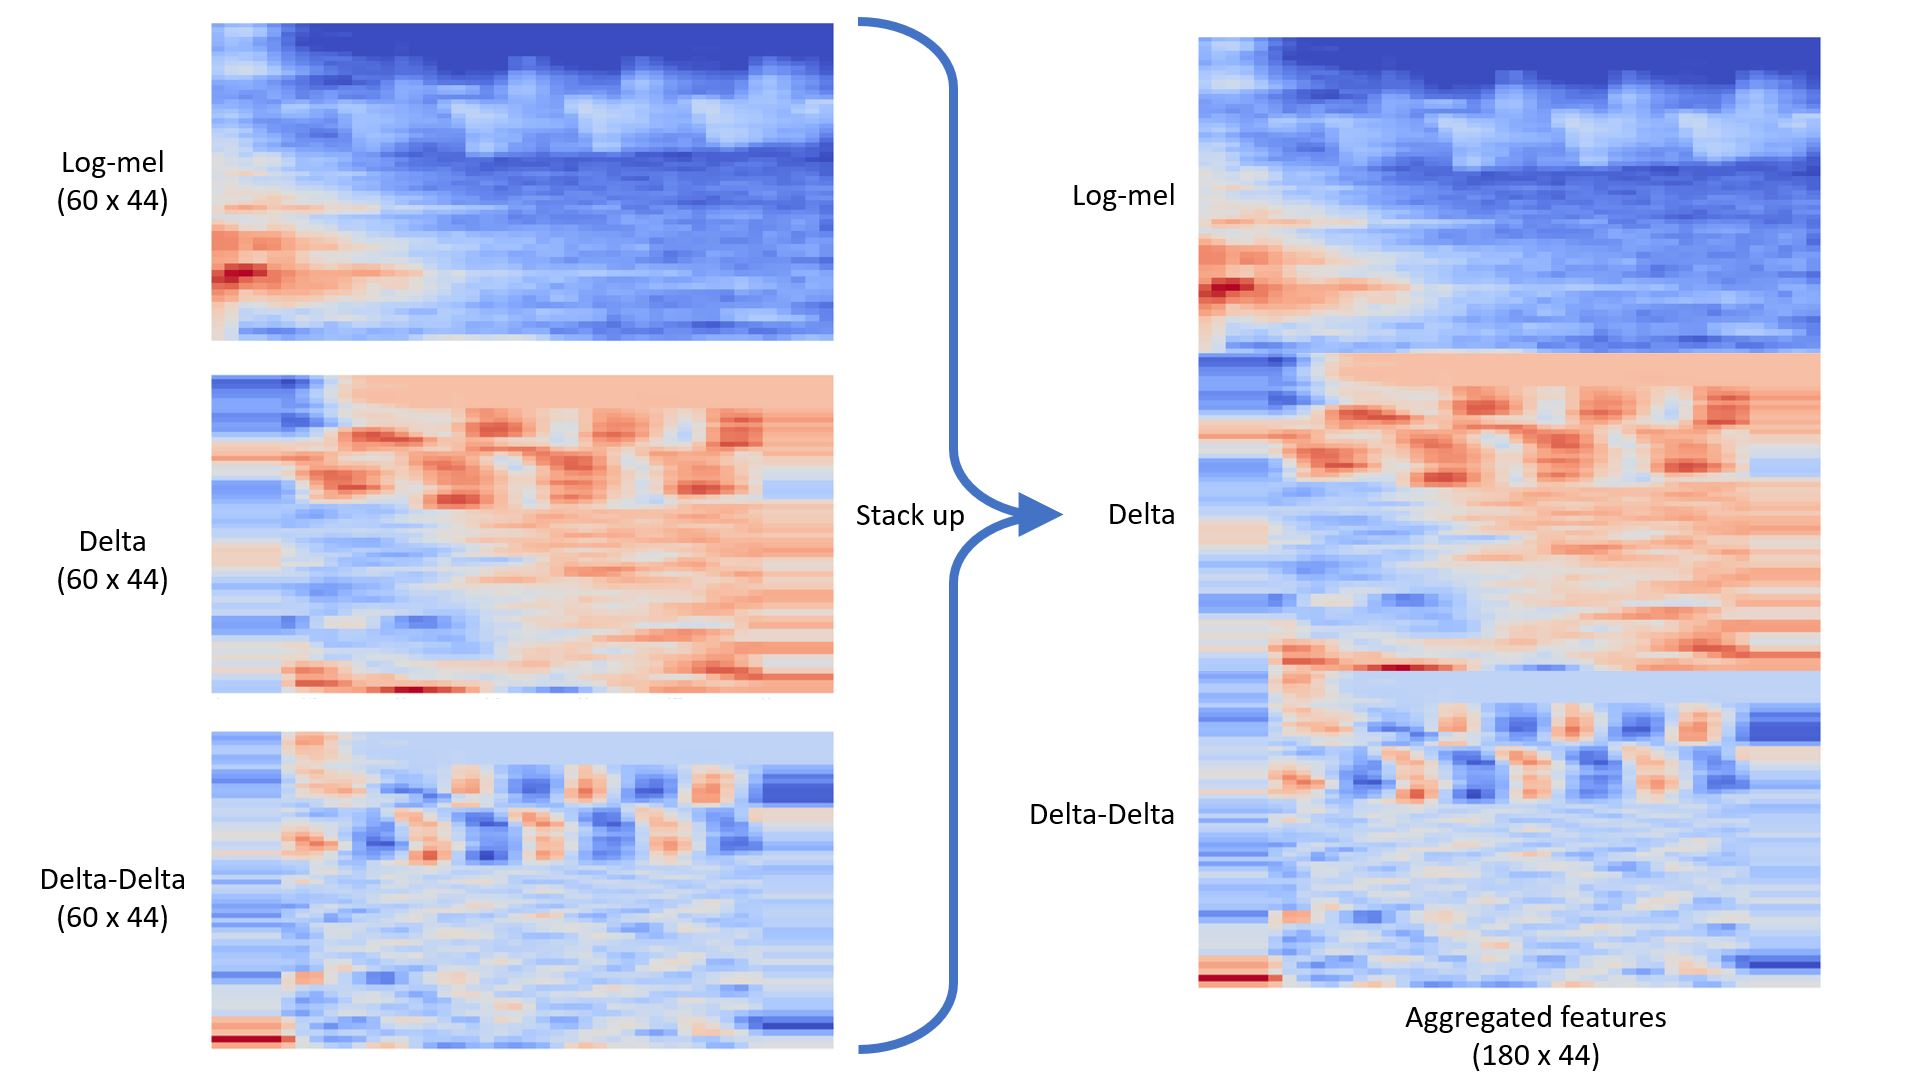
\includegraphics[width=1\textwidth]{resources/images/050-methods/Methods_feature_extraction_3_US8K.jpg}
        \smallcaption{Source: Author}
        \label{fig:methods_feature_extraction_log-mel_spectrogram}
\end{figure}

\section{TRAINING THE CLASSIFIERS}
\label{sec:methods_training_classifiers}

The initial step in training the models involved finding the best \index{hyperparameter}hyperparameters using grid search and built-in cross-validation \index{scikit-learn}\cite{scikitle61} to optimize model performance. Grid search systematically explored a predefined hyperparameter grid, testing various combinations to identify the set that yields the best performance, while built-in cross-validation was employed to assess model generalization by dividing the dataset into multiple subsets. The use of built-in cross-validation helps mitigate overfitting by providing a more robust estimate of the model performance across different data subsets, ensuring that the selected hyperparameters are likely to perform well on unseen data.

By default, the grid search splits the dataset into training and testing sets according to the parameter $cv$ (number of cross-validations), and the model is trained on the former and evaluated on the latter, repeatedly, for each combination of hyperparameters in the grid. Depending on the number of hyperparameters to be searched, this process may take a long time to execution, especially in neural networks, and therefore, although recommended in the general literature to run the built-in cross-validation with 10 sets, it was established the number of 5 sets for all models, hence 80\% for training and 20\% for testing. Once the set of optimal hyperparameters was found for each model, the final step of the training started, validating the model on a separate, unseen validation set, using the method of k-fold cross-validation, to assess its true generalization performance. 

Each of the aforementioned datasets was initially intended to undergo validation using k-fold cross-validation methods, with each dataset considering a distinct value for k as specified by their curators: ESC-10 employs 5 folds, BDLib2 utilizes 3 folds, and UrbanSound8K employs 10 folds. Figure \ref{fig:methods_training_k-fold} illustrates the process of the k-fold cross-validation using the ESC-10 dataset as an example, demonstrating that each k-fold (0 to 4) assigned in the dataset metadata was properly separated within the 10 classes. In order to compare the classifier's results accordingly, the number of k-folds for each dataset was respected.

At the end of this process, the classifier models using machine learning techniques and ensemble methods were configured with their standard parameters according to the \index{scikit-learn}scikit-learn library, except for the following \index{hyperparameter}hyperparameters:

\begin{itemize}
    \item \gls{gnb}: $ priors$ = none (Prior probabilities of the classes);
    \item \gls{svm}: $kernel$ = 'linear', $C$ = 0.50 (Regularization parameter);
    \item \gls{lr}: $solver$ = 'saga', $C$ = 0.50 (Regularization parameter), $max\_iter$ = 500 (Maximum number of iterations taken for the solver to converge);
    \item \gls{k-nn}: $n\_neighbors$ = 3, $metric$ = 'minkowski', $p$ = 2 (Power parameter for the Minkowski metric, 2 means Euclidean distance), $leaf\_size$ = 20 (Leaf size passed to BallTree or KDTree algorithm to calculate the nearest neighbors considered that 'auto' is the standard);
    \item \gls{rf}: $criterion$ = 'gini', $n\_estimators$ = 500 (The number of trees in the forest), $bootstrap$ = True (Whether bootstrap samples are used when building trees);
    \item Voting: $voting$ = 'soft' (Predicts the class label based on the argmax of the sums of the predicted probabilities).
\end{itemize}

\begin{figure}[htbp]
    \raggedright
        \caption{Process of k-fold cross-validation using the metadata of the dataset ESC-10 with 10 classes and 5 folds.}
        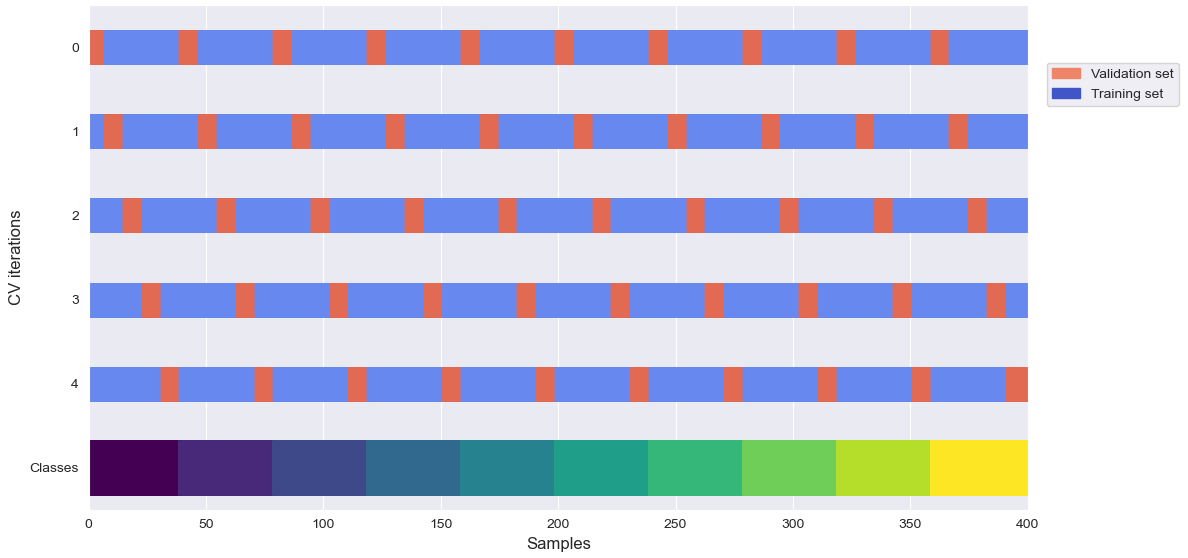
\includegraphics[width=1\textwidth]{resources/images/050-methods/Methods_training_k-fold.png}
        \smallcaption{Source: Author}
        \label{fig:methods_training_k-fold}
\end{figure}

The \gls{ann} was originally created using Kolmogorov's theorem where given any continuous function
$\phi: I^n \longrightarrow \mathbf{R}^m, \phi(\mathbf{x})=\mathbf{y}$, where $I$ is the closed unit interval $[0,1]$ representing the classes, and therefore $I^n$ is the $n$ dimensional unit cube, $\phi$ can be implemented exactly by a 3 layer neural network having $n$ processing elements in the first input layer ($x$), followed by $(2 n+1)$ processing elements (neurons) in the hidden layer, and $m$ processing elements in the output layer ($y$) \cite{Hecht-Nielsen1987}. The network was built using the \index{Keras}Keras sequential model to define an \gls{mlp} with the first dense layer receiving as input an array with 375 features (parameterized with \gls{pca} when requested) and the \gls{relu} activation function. The second and third dense layers were hidden, with 375 neurons and 750 neurons, respectively, both using the \gls{relu} activation function. To improve the model accuracy proposed by Hecht-Nielsen, one additional hidden dense layer was added based on the grid search and built-in cross-validation results. A dropout layer with 20\% rate was also added after each hidden layer to improve generalization, prevent overfitting, and make the model more robust by introducing randomness during training.

The final dense layer with $n$ neurons — one for each class, $n=6$ for the dataset US8K\_AV and $n=10$ for the datasets ESC-10, BDLib2, and \gls{us8k} — is utilized for the classification task using the \textbf{softmax} activation function to assign probabilities to each class in the output layer. The hyperparameters used in the grid search to achieve this model configuration, illustrated by Figure \ref{fig:methods_training_ANN_architecture} and Figure \ref{fig:methods_training_ANN_architecture_jupyter_notebook}, were $loss$ = 'categorical\_crossentropy', and the Adam optimizer with $learning\_rate$ = 0.0001, $beta\_1$ = 0.5 (The exponential decay rate for the 1\textsuperscript{st} moment estimates), $beta\_2$ = 0.999 (The exponential decay rate for the 2\textsuperscript{nd} moment estimates), $epsilon$ = $10^{-7}$ (A small constant for numerical stability), and $amsgrad$ = True (Whether to apply AMSGrad variant \cite{Reddi2018} of this algorithm). 


\begin{figure}[htbp]
    \raggedright
        \caption{ANN architecture utilized in the benchmark datasets.}
        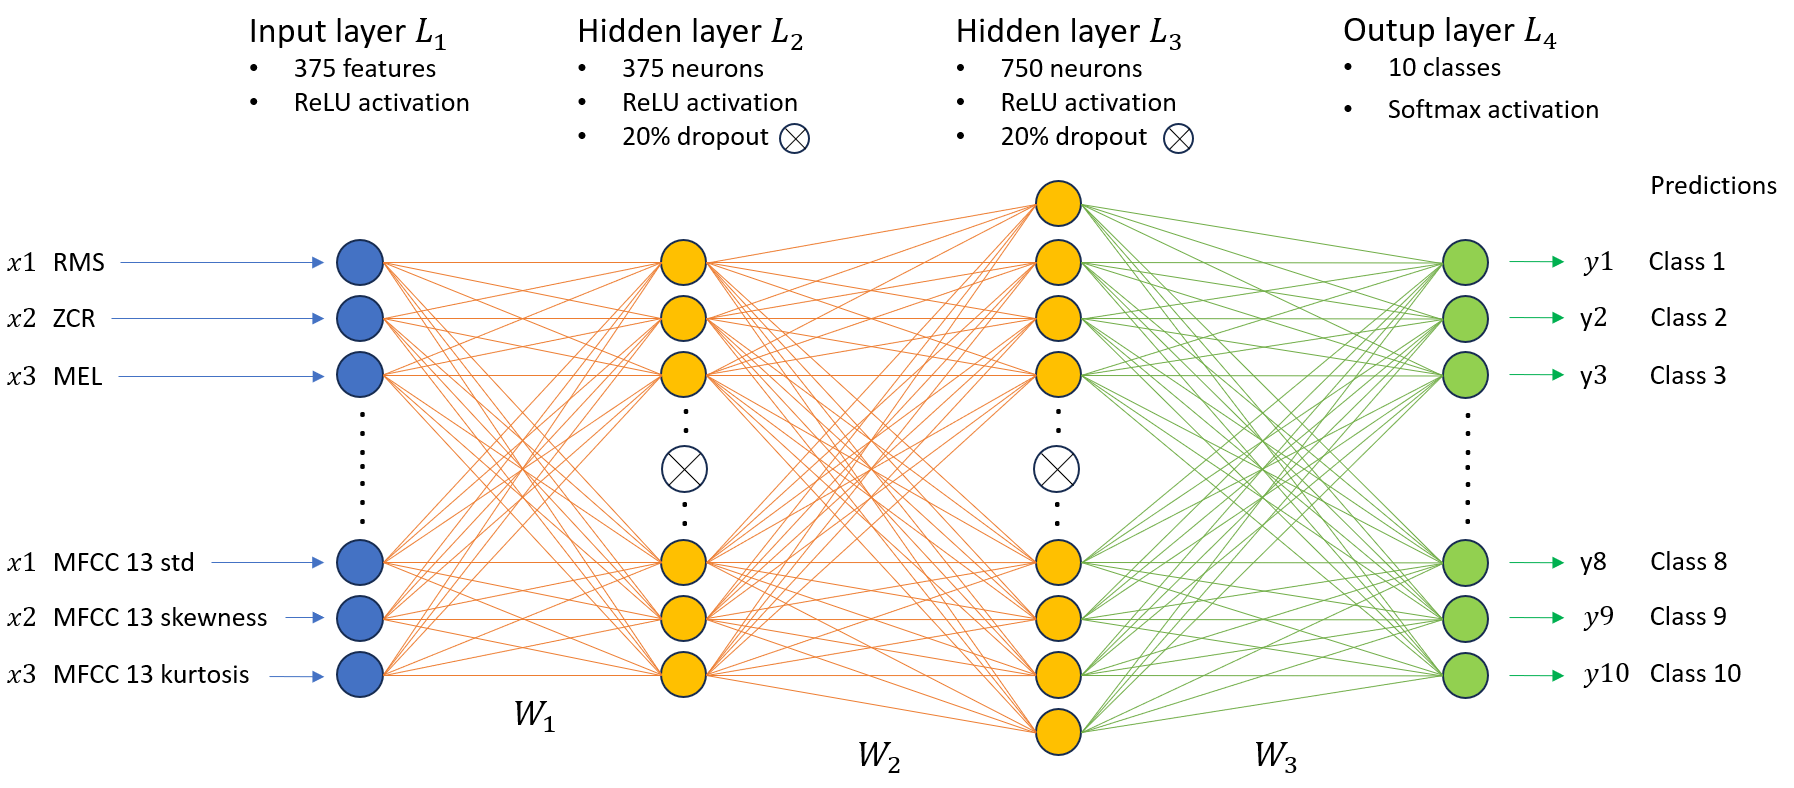
\includegraphics[width=1\textwidth]{resources/images/050-methods/Methods_training_ANN_architecture.png}
        \smallcaption{Source: Author}
        \label{fig:methods_training_ANN_architecture}
\end{figure} 


\begin{figure}[htbp]
    \raggedright
        \caption{ANN model summary from Jupyter notebook utilized in the benchmark datasets.}
        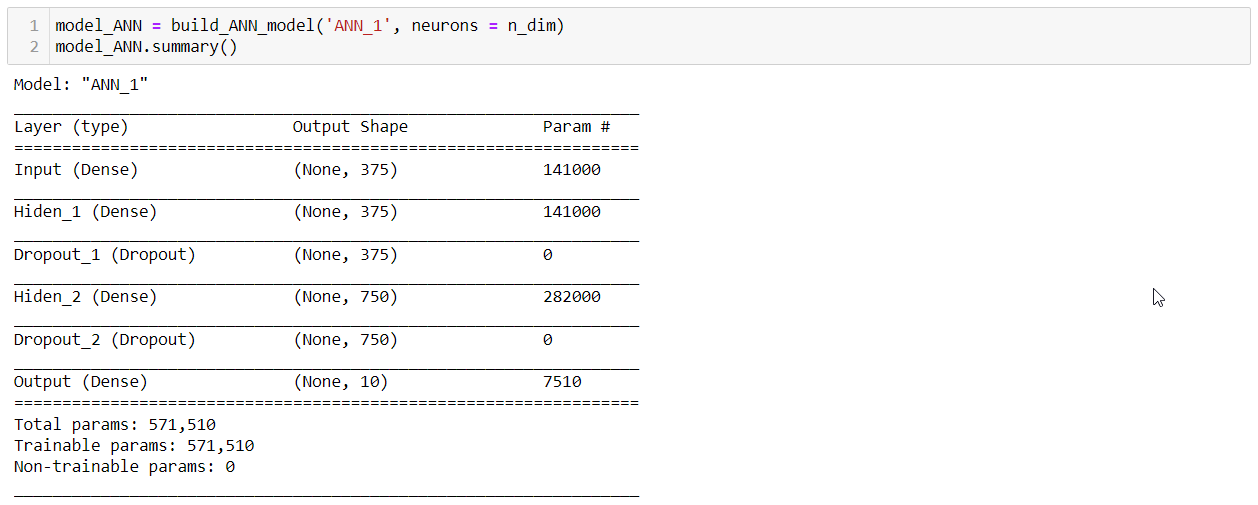
\includegraphics[width=1\textwidth]{resources/images/050-methods/Methods_training_ANN_architecture_jupyter_notebook.png}
        \smallcaption{Source: Author}
        \label{fig:methods_training_ANN_architecture_jupyter_notebook}
\end{figure} 


A second round of grid search was performed to find the best parameters for the batch size and epochs, and this was implemented together with an early stop process. Ultimately, the values considered were: $batch\_size = 20$, $epochs$ = 350 and $EarlyStopping$ with $monitor$ = 'val\_accuracy', $min\_delta$ = 0.0001, $patience$ = 150, and $restore\_best\_weights$ = True. As illustrated in Figure \ref{fig:methods_training_ANN_loss_and_accuracy_graphs}, the \gls{ann} model achieved a stable and rather well-generalized behavior during the built-in cross-validation process.


\begin{figure}[htbp]
    \raggedright
        \caption{Loss and accuracy graphs of the implemented ANN model.}
        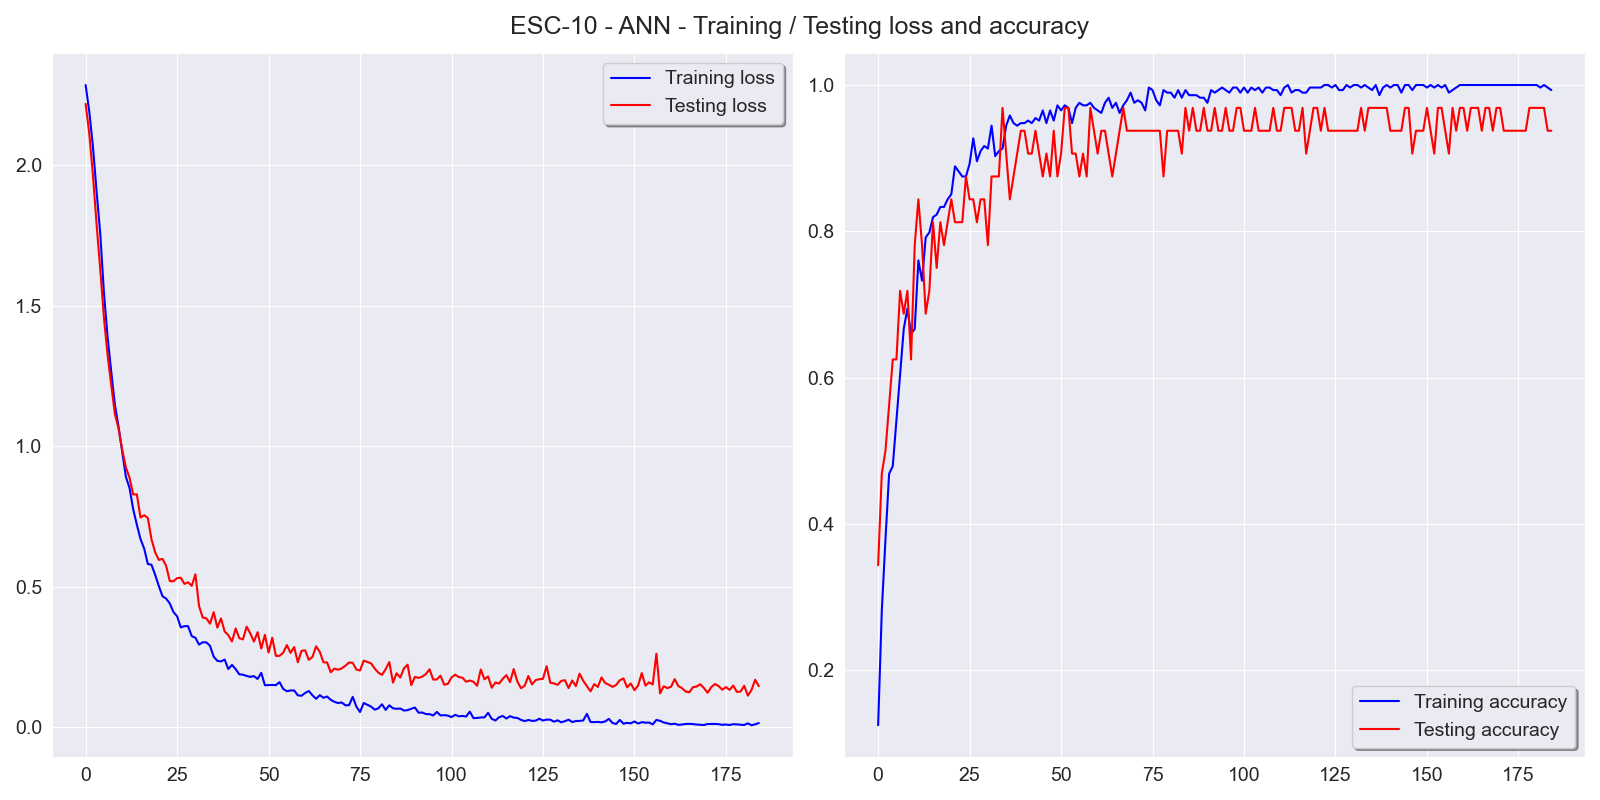
\includegraphics[width=1\textwidth]{resources/images/050-methods/Methods_training_ANN_loss_accuracy.png}
        \smallcaption{Source: Author}
        \label{fig:methods_training_ANN_loss_and_accuracy_graphs}
\end{figure} 

The architecture of the \gls{cnn} 1D model illustrated in Figure \ref{fig:methods_training_CNN_1D_architecture} and summarized by the Jupyter notebook in Figure \ref{fig:methods_training_CNN_1D_architecture_jupyter_notebook} consisted of several layers, compiled with a categorical cross-entropy loss function, Adamax optimizer, and accuracy as the evaluation metric:

\begin{figure}[htbp]
    \raggedright
        \caption{CNN 1D architecture utilized in the benchmark datasets.}
        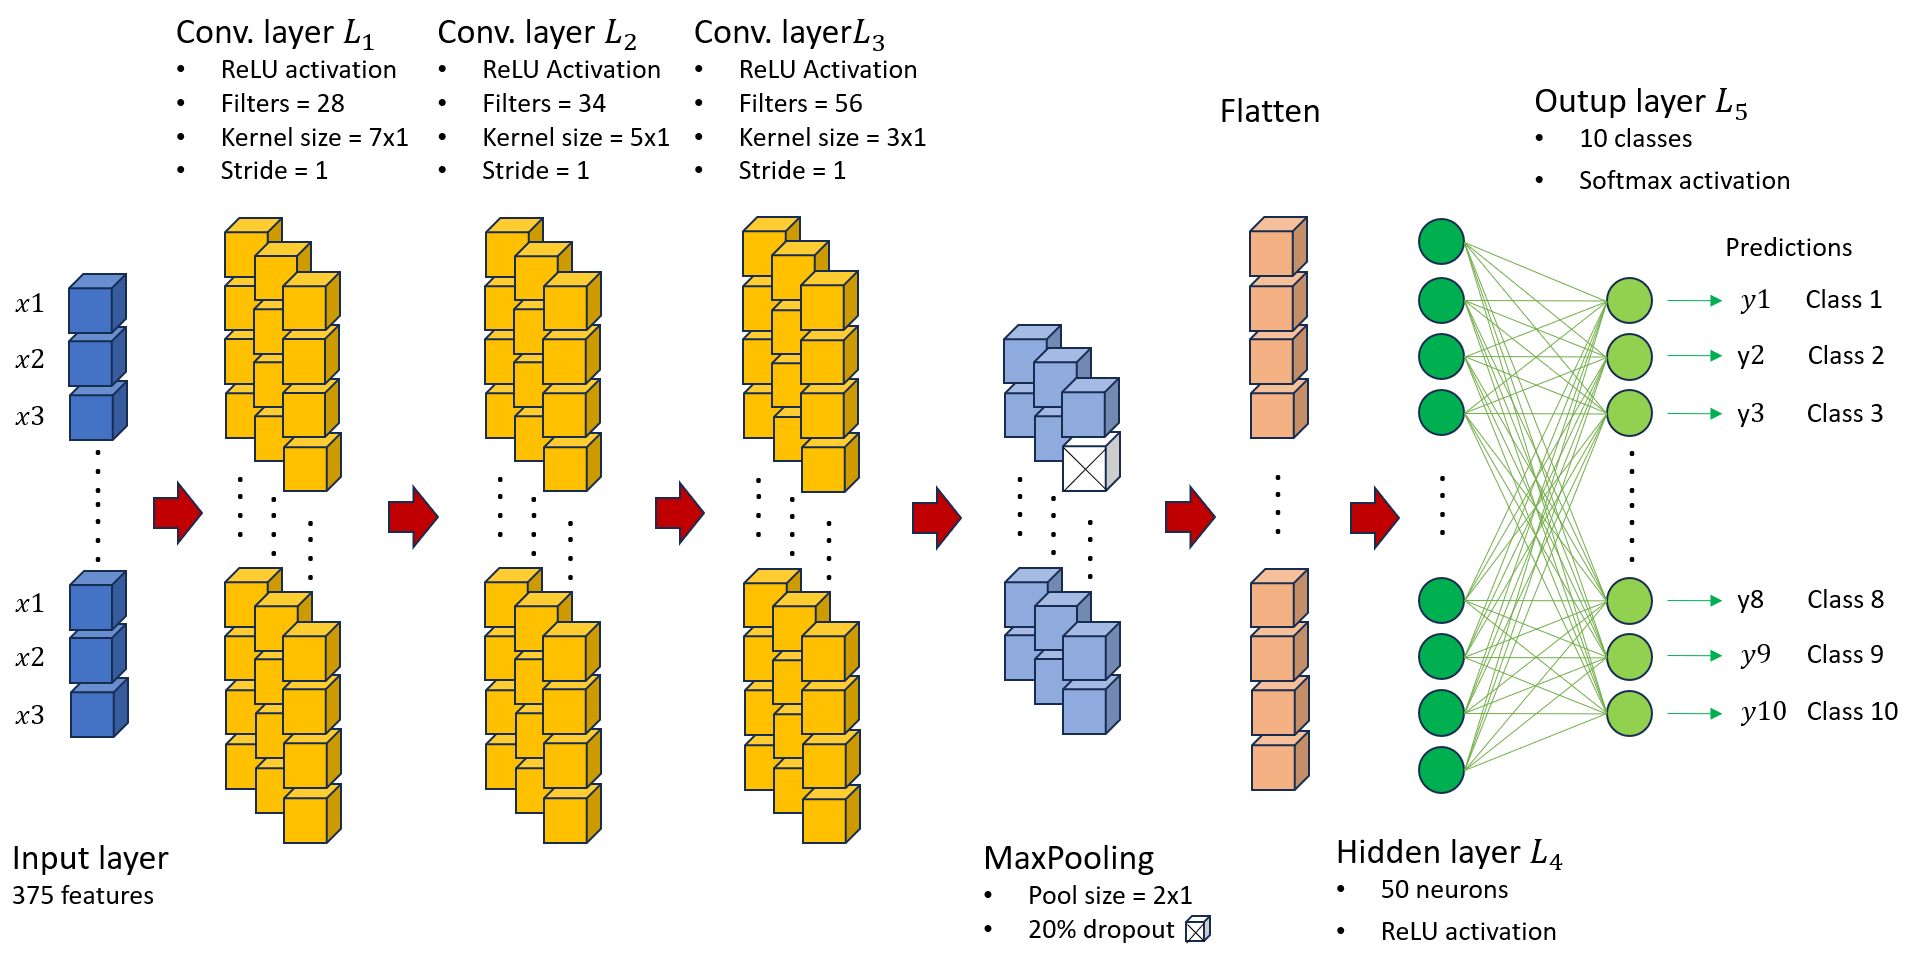
\includegraphics[width=1\textwidth]{resources/images/050-methods/Methods_training_CNN1D_architecture.png}
        \smallcaption{Source: Author}
        \label{fig:methods_training_CNN_1D_architecture}
\end{figure} 

\begin{itemize}
    \item Conv1D\_1: the first convolutional layer has 28 filters with a kernel size of 7x1, and it uses the \gls{relu} activation function, receiving as input an array with 375 features;
    \item Conv1D\_2: this is the second convolutional layer with 34 filters, and kernel size of 5x1. It also uses the \gls{relu} activation function and applies L2 regularization to the kernel with 0.001 and to the bias with 0.01. $Padding$ is set to 'same' with $stride$ as default (1) to ensure the output size matches the input size;
    \item Conv1D\_3: this is the last convolutional layer. It has 56 filters with a kernel size of 3x1. The same parameters of the second convolutional layer are used for the activation function and L2 regularization to the kernel and bias;
    \item MaxPooling1D\_3: this layer performs max pooling with a pool size of 2x1, reducing the dimensionality of the data by taking the maximum value within each window of size 2x1;
    \item Dropout\_1: to reduce overfitting, this layer randomly sets 20\% of the input units to 0 at each update during training; 
    \item Flatten\_5: to prepare the data for the next step, this layer reshapes the output of the previous layer into a one-dimensional vector;
    \item Dense: this layer is fully-connected to the previous layer with 50 neurons; 
    \item Output: finally, the classification task is performed in this layer. It has a number of neurons equal to the number of output classes (6 or 10), and it uses the softmax activation function to output probabilities for each class.
\end{itemize}

\begin{figure}[htbp]
    \raggedright
        \caption{CNN 1D model summary from Jupyter notebook utilized in the benchmark datasets.}
        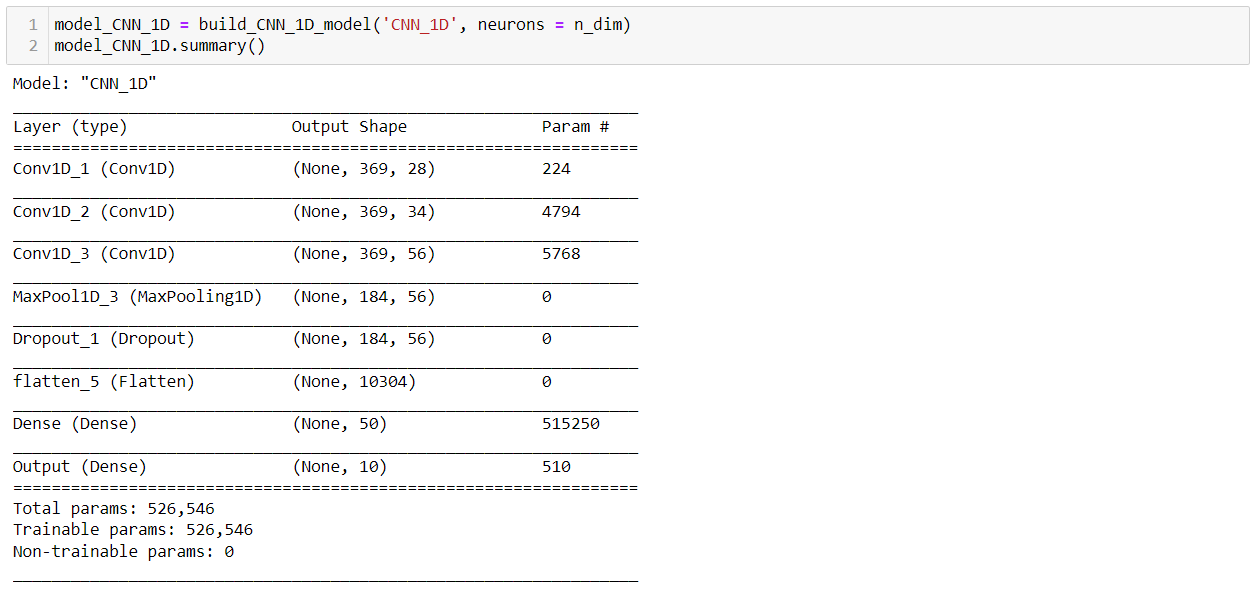
\includegraphics[width=1\textwidth]{resources/images/050-methods/Methods_training_CNN1D_architecture_jupyter_notebook.png}
        \smallcaption{Source: Author}
        \label{fig:methods_training_CNN_1D_architecture_jupyter_notebook}
\end{figure} 

In the same way as the \gls{ann}, a grid search was performed to find the batch size and epochs that yield the highest accuracy, implemented together with an early stop process. In the final stages, the values considered were: $batch\_size = 20$, $epochs$ = 150 and $EarlyStopping$ with $monitor$ = 'val\_accuracy', $min\_delta$ = 0.0001, $patience$ = 50, and $restore\_best\_weights$ = True. Figure \ref{fig:methods_training_CNN_1D_loss_and_accuracy_graphs} depicts a robust model that achieved the highest accuracy with just a few epochs. The early stop was triggered during the built-in cross-validation between 50 and 70 epochs.


\begin{figure}[htbp]
    \raggedright
        \caption{Loss and accuracy graphs of the implemented CNN 1D model.}
        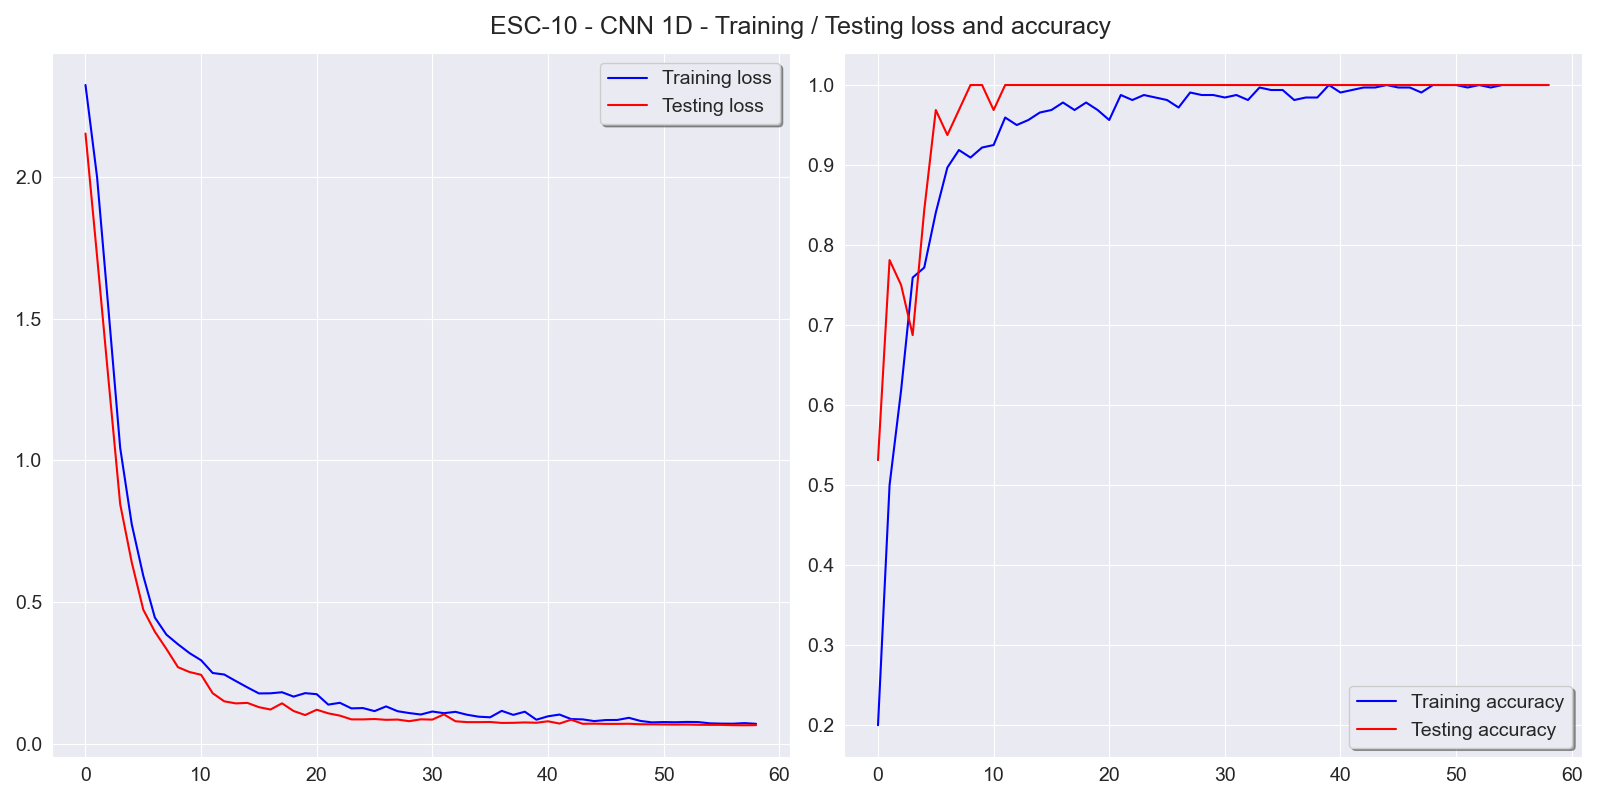
\includegraphics[width=1\textwidth]{resources/images/050-methods/Methods_training_CNN1D_loss_accuracy.png}
        \smallcaption{Source: Author}
        \label{fig:methods_training_CNN_1D_loss_and_accuracy_graphs}
\end{figure} 


During this phase of the study, several architectures for the \gls{cnn} 2D model were examined, including those proposed by \textcite{Piczak2015}, \textcite{Su2020}, \textcite{Luz2021}, and \textcite{Chu2023}. The architecture that exhibited the best performance was adapted from \textcite{Su2020}. However, this model was modified to utilize four convolutional layers, in contrast to the six layers in the original design. Additionally, modifications were made to the stride values in specific layers, and additional dropout layers were incorporated. The final model (Figure \ref{fig:methods_training_CNN_2D_architecture}) was compiled using a categorical cross-entropy loss function, a \gls{sgd} optimizer (with a learning rate of 0.001 and momentum of 0.9), and accuracy as the evaluation metric:

\begin{figure}[htbp]
    \raggedright
        \caption{CNN 2D architecture utilized in the experiments. Specific illustration for the US8K\_AV dataset with 6 output classes.}
        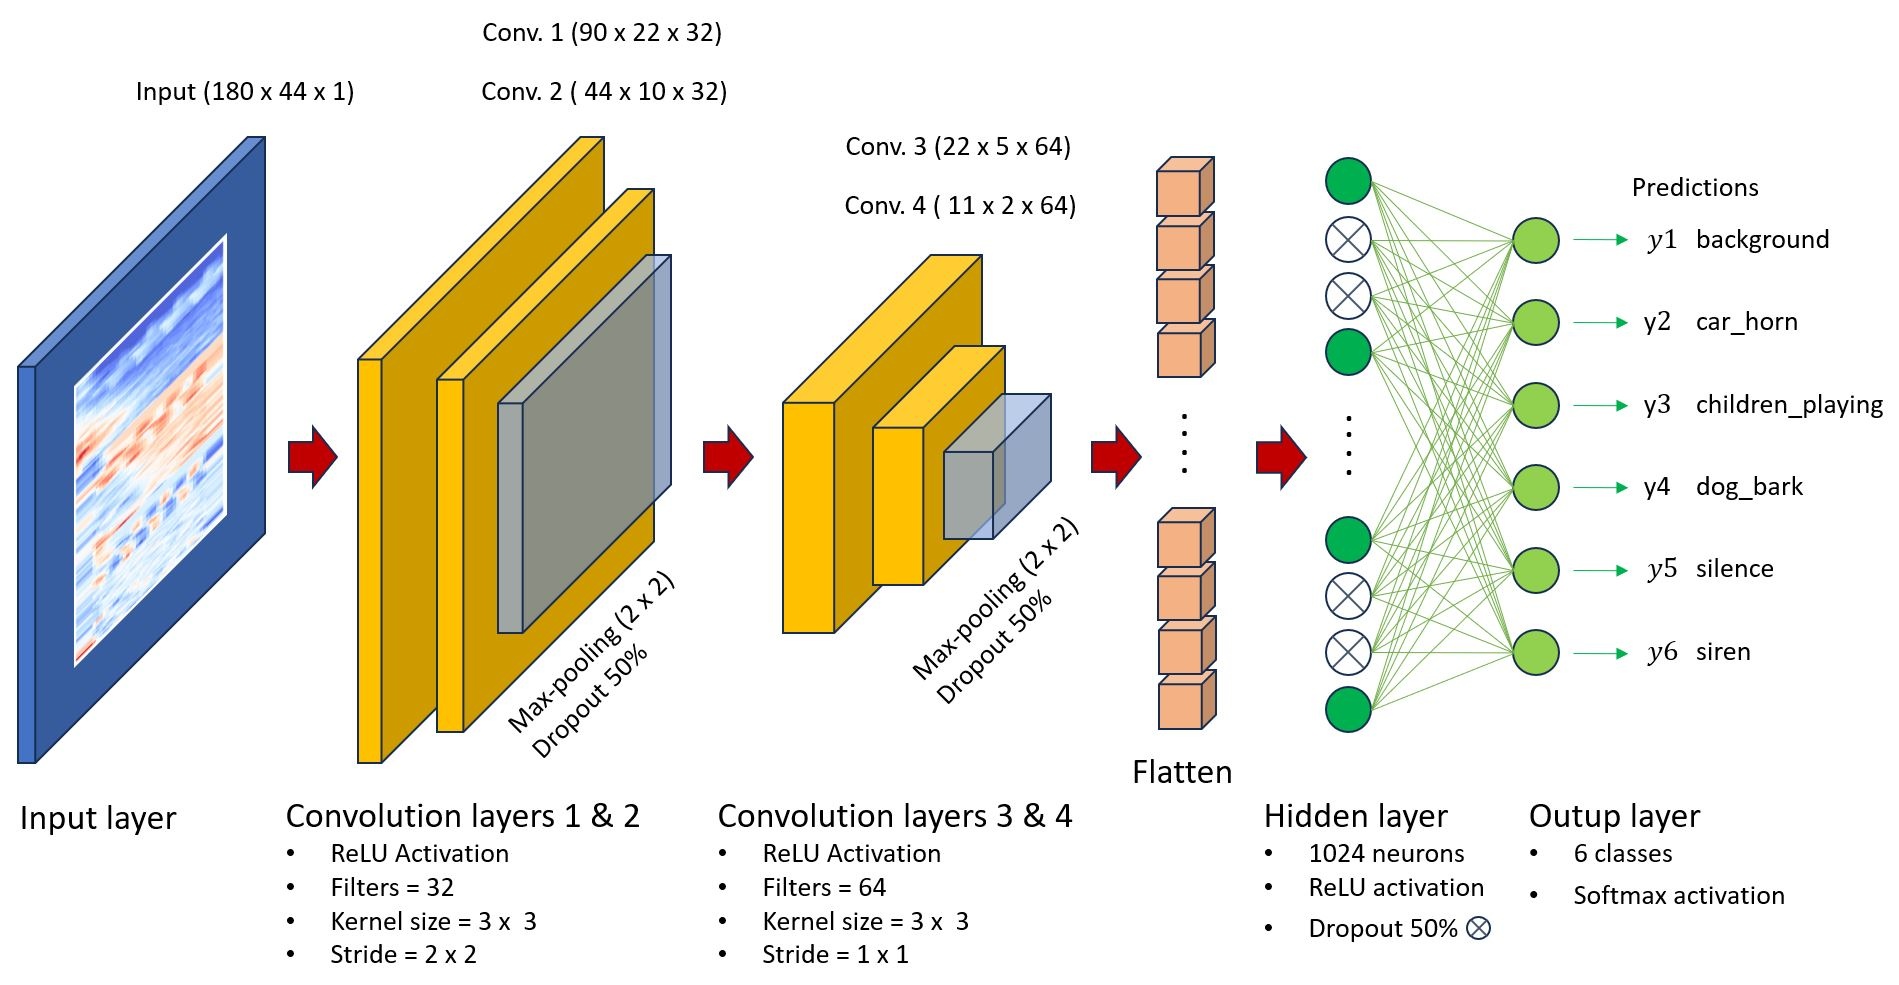
\includegraphics[width=1\textwidth]{resources/images/050-methods/Methods_training_CNN2D_architecture.jpg}
        \smallcaption{Source: Author}
        \label{fig:methods_training_CNN_2D_architecture}
\end{figure} 

\begin{itemize}
    \item The first convolutional layer comprises 32 filters with a kernel size of 3x3 and a stride of 2x2, utilizing the \gls{relu} activation function, followed by batch normalization;
    \item The second convolutional layer mirrors the first one but is followed by a max-pooling layer with a pool stride of 2x2 to reduce the dimensions of the convolutional feature maps and includes a dropout rate of 50\% to mitigate overfitting;
    \item The third convolutional layer consists of 64 filters with a kernel size of 3x3 and a stride of 1x1, employing the \gls{relu} activation function, followed by batch normalization;
    \item The fourth convolutional layer is identical to the third one but is succeeded by a max-pooling layer with a pool stride of 2x2 and a dropout rate of 50\%;
    \item A flatten layer reshapes the output from the previous layer into a one-dimensional vector in preparation for subsequent processing;
    \item A fully-connected dense layer with 1,024 neurons is added before the final output, followed by another dropout layer set at 50\%;
    \item The final classification task is performed in the last layer, which contains neurons equal to the number of output classes (6 or 10) and uses the softmax activation function to output probabilities for each class;
\end{itemize}

A grid search was conducted to determine the optimal batch size and number of epochs that would yield the highest accuracy. This process was implemented alongside an early stopping mechanism. The implemented parameters were: $batch\_size = 32$, $epochs$ = 100 and $EarlyStopping$ with $monitor$ = 'val\_accuracy', $min\_delta$ = 0.0001, $patience$ = 20, and $restore\_best\_weights$ = True. Figure \ref{fig:methods_training_CNN_2D_loss_and_accuracy_graphs} illustrates that the model continued to learn and may have achieved better performance if trained for additional epochs since early stopping was never triggered during built-in cross-validation. Nonetheless, limiting the training to 100 epochs was considered sufficient for this study.


\begin{figure}[htbp]
    \raggedright
        \caption{Loss and accuracy graphs of the implemented CNN 2D model.}
        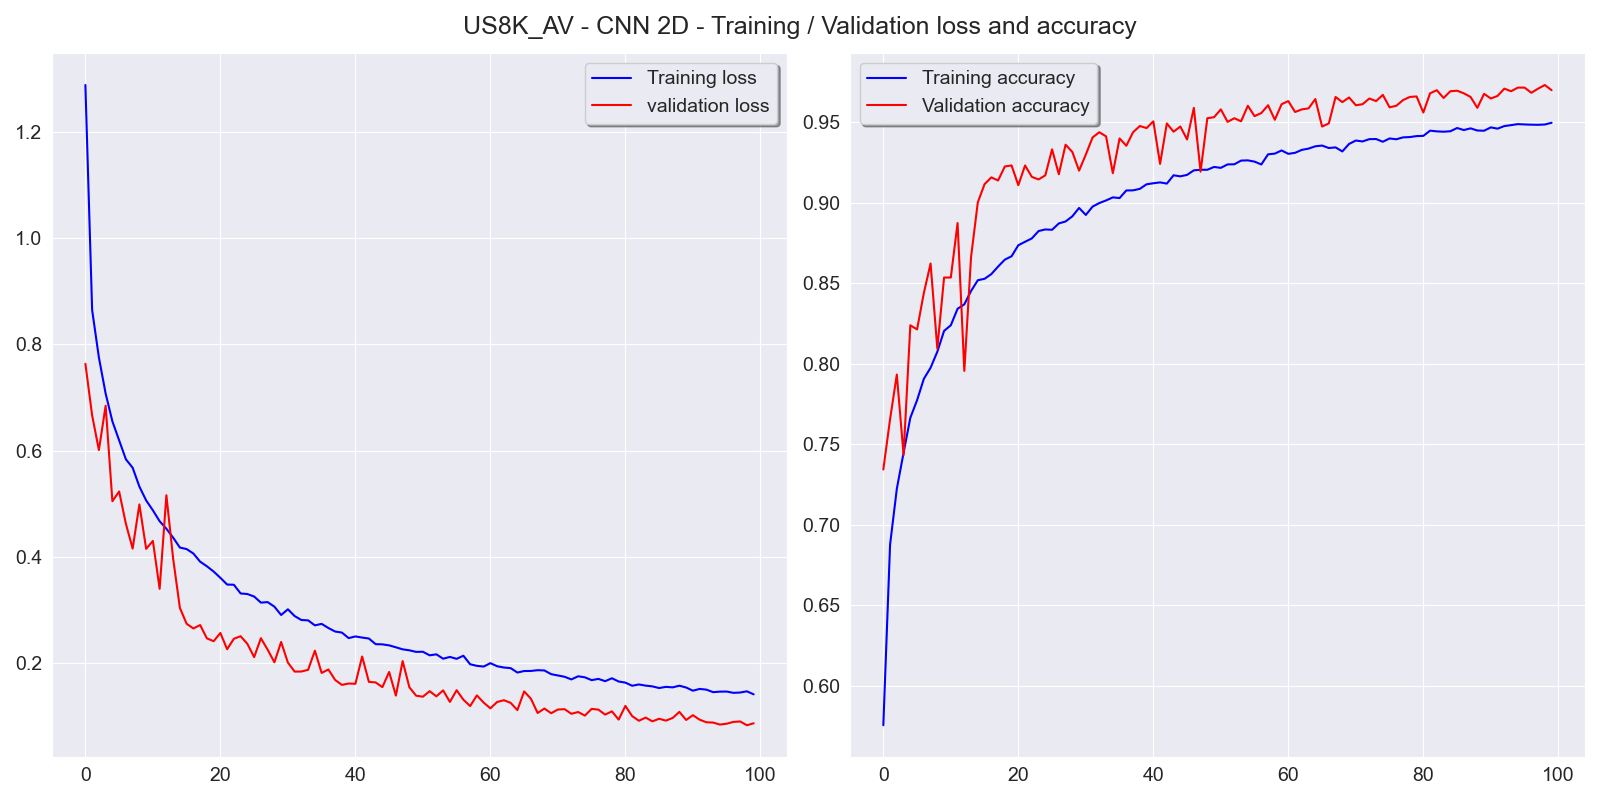
\includegraphics[width=1\textwidth]{resources/images/050-methods/Methods_training_CNN2D_loss_accuracy.png}
        \smallcaption{Source: Author}
        \label{fig:methods_training_CNN_2D_loss_and_accuracy_graphs}
\end{figure} 


\section{EVALUATION}
\label{sec:methods_evaluation}

Once the training is completed, the evaluation phase starts, initially stationary as illustrated in the methodology diagram (Training / Classification flow), and lastly mobile (Evaluation flow), in the practical scenario of a regular passenger vehicle, considering factors like ambient noise, changing environmental conditions, and the need for instantaneous responses.

The C-Bots utilized in the living laboratory are equipped with ReSpeaker Mic Array v2.0 \cite{ReSpeake72} installed in the AVATAR head (Figure \ref{fig:methods_evaluation_AVATAR_ReSpeaker}), connected to the AVATAR \gls{ecu}, which is used for speech recognition, among other functions. The ReSpeaker contains 4 high-performance digital microphones (ST MP34DT01TR-M), with a sensitivity of -26 \gls{db}FS (Omnidirectional), acoustic overload point of 120 \gls{db} \gls{spl}, maximum sampling rate of 16 \gls{k}\gls{hz}, and speech recognition algorithm on-chip, including support to far-field voice capture. The AVATAR \gls{ecu} is a Raspberry Pi connected to the vehicle \gls{ee} architecture via \gls{can} and Ethernet, and according to the C-Bot system engineer, the \gls{esr} algorithm could be implemented on this module or in another high-performance computing module of the vehicle, and its output information published via ROS2. 

\begin{figure}[htbp]
    \raggedright
        \caption{Illustration of the ReSpeaker Mic Array v2.0 installed in the AVATAR of the C-Bot.}
        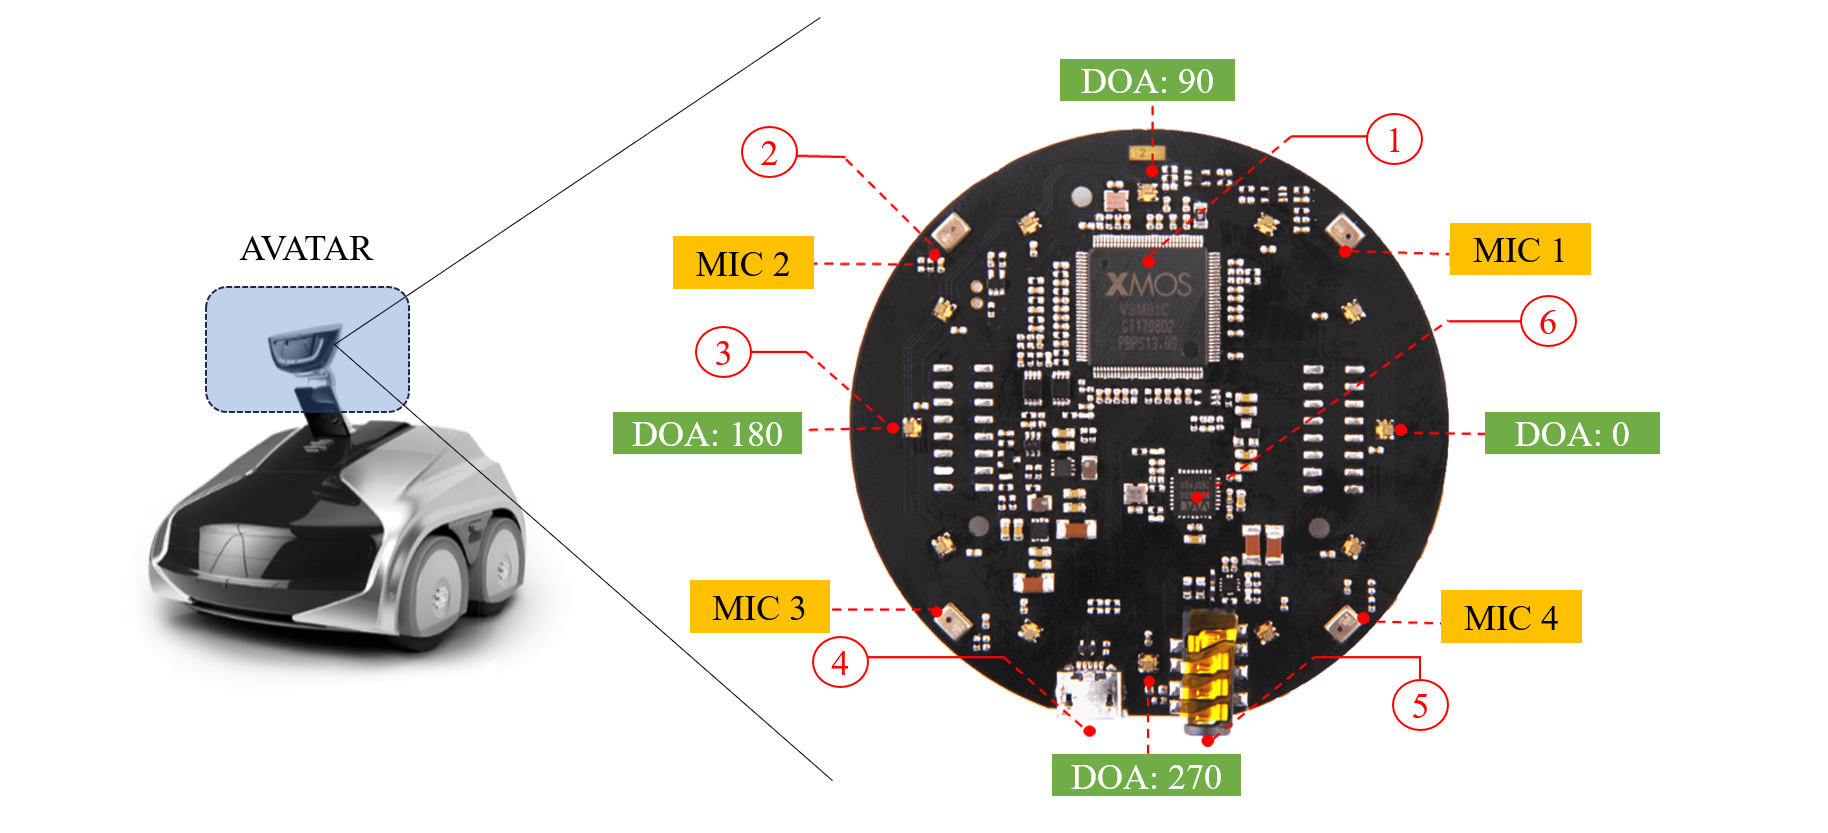
\includegraphics[width=.85\textwidth]{resources/images/050-methods/Methods_evaluation_microphone_ReSpeaker_Mic_Array_v2.0.png}
        \smallcaption{Source: Author, "adapted from" \textcite{ReSpeake72} }
        \label{fig:methods_evaluation_AVATAR_ReSpeaker}
\end{figure}

As described in subsection \ref{subsec:objectives_specifics}, the C-Bot hardware is not available in Brazil for testing, therefore, the best-performing model was deployed in a high-end general-purpose platform identical to the AVATAR, denoted as Raspberry Pi 4 model B \cite{Raspberry2023}, hereinafter named only as Raspberry Pi, with 8 \gls{g}\gls{b} SDRAM and Quad core Cortex-A72 (ARM v8) 64-bit SoC @1.8 \gls{g}\gls{hz}. 

Before the evaluation flow took place in the VW UP, an experiment was performed indoors to evaluate the soundness of the predictive algorithm. This experimental setup involved connecting a single microphone directly to a Raspberry Pi to facilitate live prediction with an interval of 1 \gls{s}. The Raspberry Pi housed both the audio clips employed by the algorithm and the vectors for prediction results, alongside recording the total prediction time. Concurrently, an identical microphone was connected to a notebook to record audio continuously. Both recordings were initiated simultaneously to ensure temporal alignment, as illustrated in Figure \ref{fig:methods_evaluation_indoor_experiment}.

\begin{figure}[htbp]
    \raggedright
        \caption{Setup of the indoor experiment using the Raspberry Pi and the notebook.}
        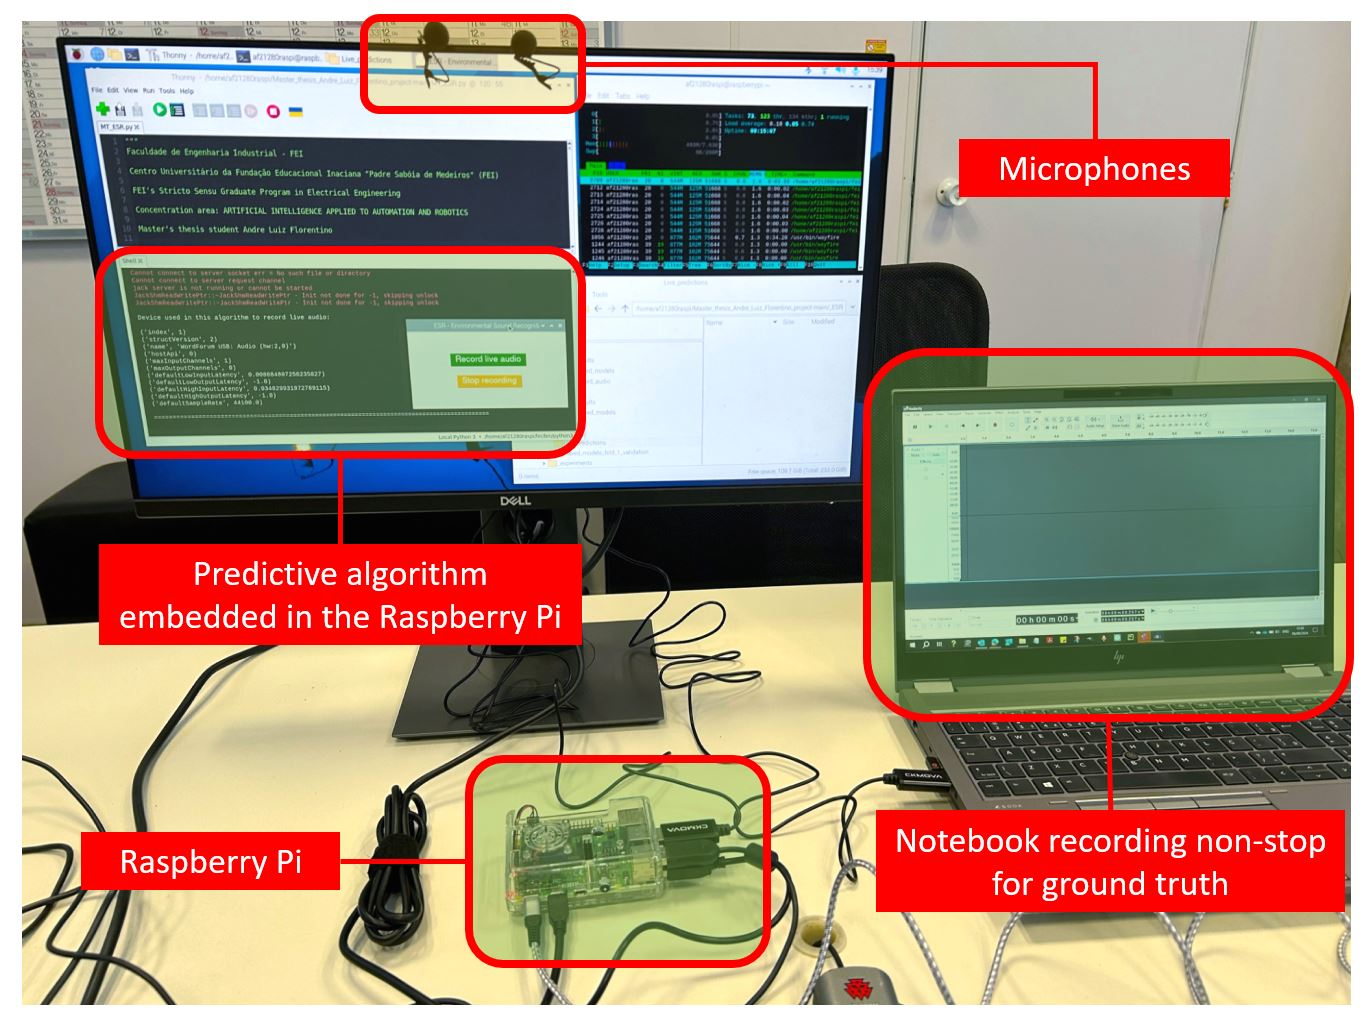
\includegraphics[width=.8\textwidth]{resources/images/050-methods/Methods_evaluation_indoor.jpg}
        \smallcaption{Source: Author}
        \label{fig:methods_evaluation_indoor_experiment}
\end{figure}

The sound source, emanating from an iPhone 11 positioned 5 meters away from the microphones, had a duration of 120 \gls{s}. For the creation of ground truth labels, the continuous audio recorded in the notebook was processed using the software Audacity \cite{Audacity2024}. Initial labels were generated according to the evaluated class, segmented into equal intervals of 1 \gls{s} each. Silence periods were automatically identified within a range of -20 \gls{db} to -30 \gls{db}, contingent upon the class under evaluation. Subsequently, these labels underwent manual adjustment through auditory inspection, ensuring accuracy by comparing the labeled segments with identified silence periods (Figure \ref{fig:methods_evaluation_audacity_ground_truth}).

This approach ensured that the ground truth labels were precisely aligned with the actual audio events, thereby providing a reliable benchmark for evaluating the performance of the predictive algorithm in real-time conditions.

\begin{figure}[htbp]
    \raggedright
        \caption{Creation of the ground truth labels using software Audacity.}
        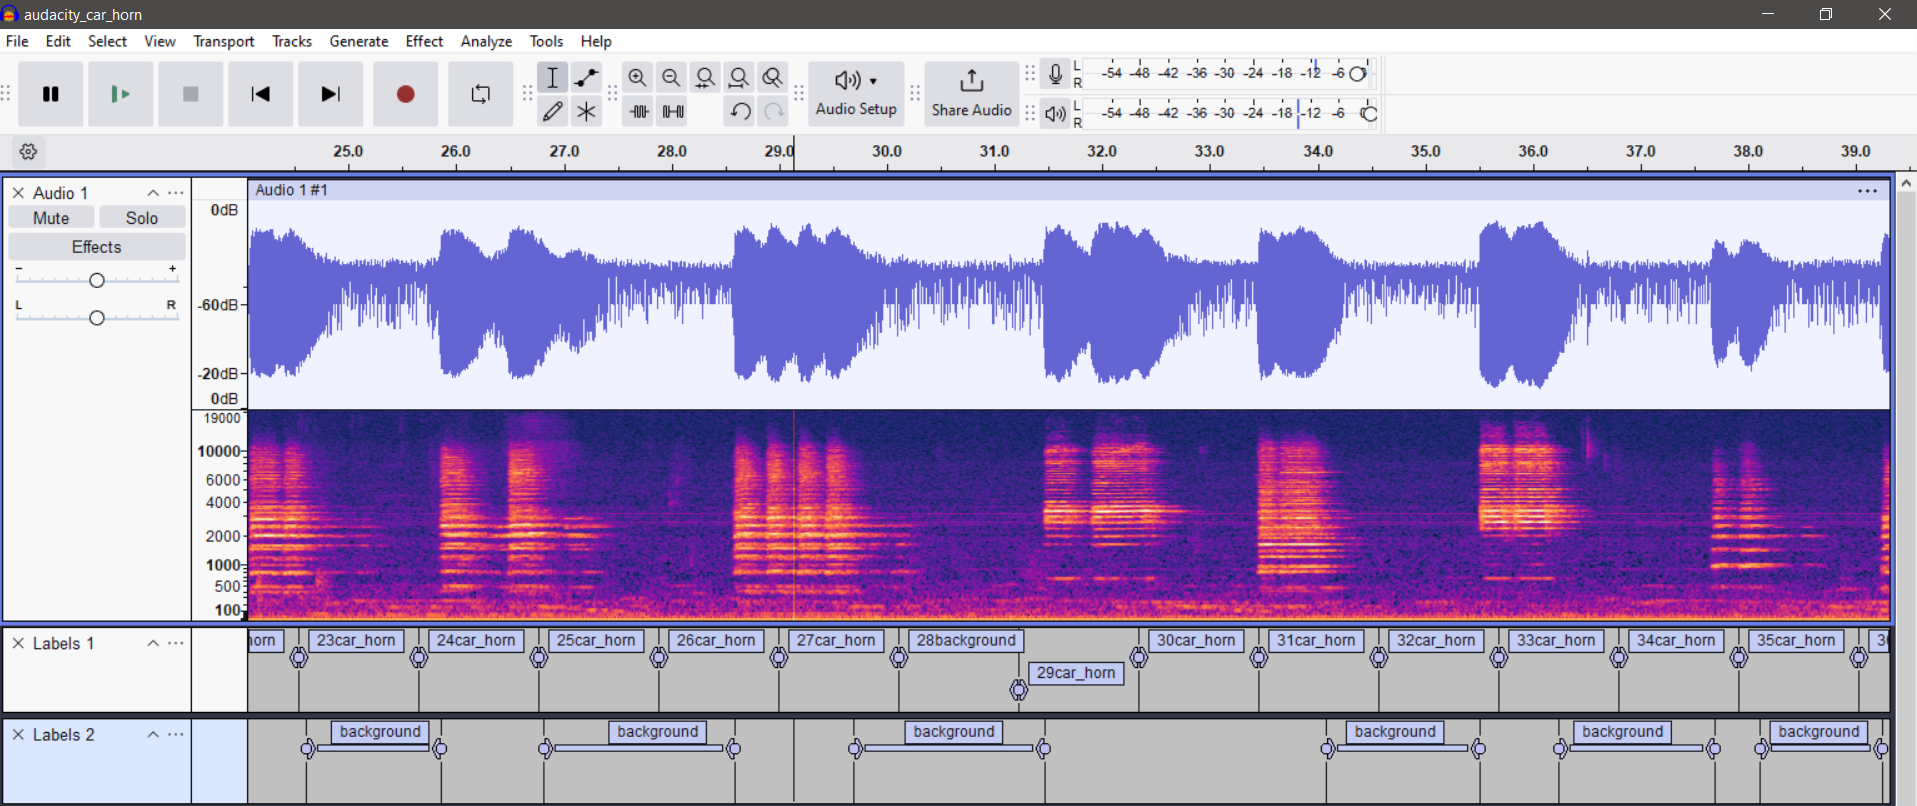
\includegraphics[width=1\textwidth]{resources/images/050-methods/Methods_evaluation_audacity_ground_truth.png}
        \smallcaption{Source: Author}
        \label{fig:methods_evaluation_audacity_ground_truth}
\end{figure}

The evaluation flow was conducted inside of the VW UP, however, the installed microphone illustrated by Figure \ref{fig:methods_evaluation_microphone_aftersales_and_VW_UP} (b) manufactured by the company BURY, with hypercardioid characteristics, electret type, output level Ua (Meß) of 67 mVeff $\pm$3 \gls{db}, acoustic pressure pMeß of 0.1 Pa, and frequency response not informed \cite{BURY2024} was replaced by a lapel microphone model USB Lavalier LUM2 series, condenser type, omnidirectional, with a frequency response of 50 Hz to 20 kHz, signal-to-noise ratio 50 dB SPL, and sensitivity of -34 dB ±3 dB \cite{CKMOVA2021} as depicted in Figure \ref{fig:methods_evaluation_microphone_aftersales_and_VW_UP} (a).

The approach employed in the indoor experiments was similarly applied to the outdoor experiments (Figure \ref{fig:methods_evaluation_outdoor_experiment}), nevertheless, due to the direct connection between the Raspberry Pi and the notebook via the USB-C port and the additional latency introduced into the system through this connection, the total prediction time for these experiments was excluded from consideration. Moreover, it was not possible to start both applications simultaneously (live prediction in the Raspberry Pi and continuous audio for the ground truth in the notebook), and therefore, a starting and ending flag were established using voice command to manually synchronize the audios afterward in the software Audacity.

\begin{figure}[htbp]
    \raggedright
        \caption{Microphone utilized in the experiments.}
        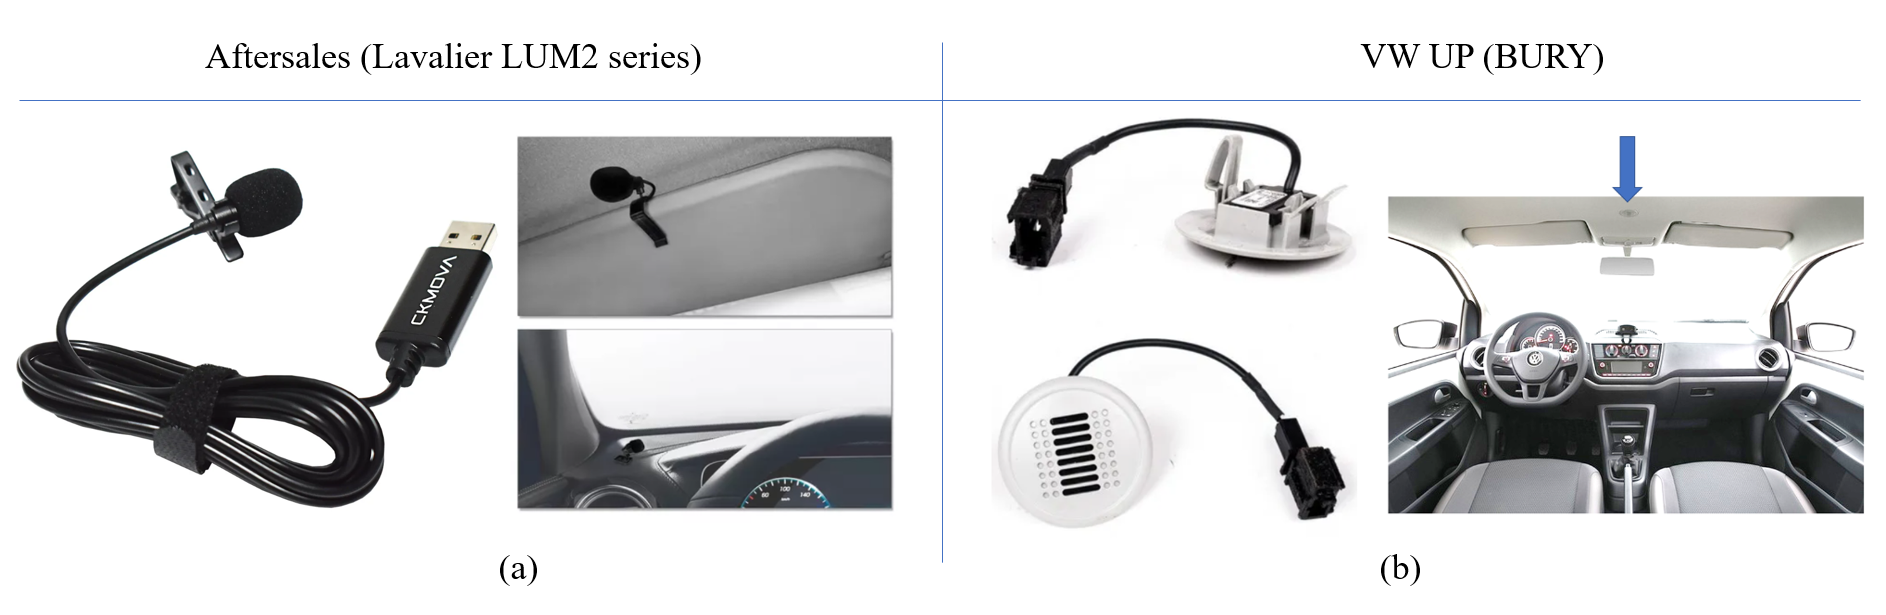
\includegraphics[width=1\textwidth]{resources/images/050-methods/Methods_evaluation_microphone_aftersales_VW_UP.png}
        \smallcaption{Source: Author, "adapted from" \textcite{Roadstar2021} and \textcite{BURY2024} }
        \label{fig:methods_evaluation_microphone_aftersales_and_VW_UP}
\end{figure}

\begin{figure}[htbp]
    \raggedright
        \caption{Setup of the outdoor experiment using the Raspberry Pi and the notebook.}
        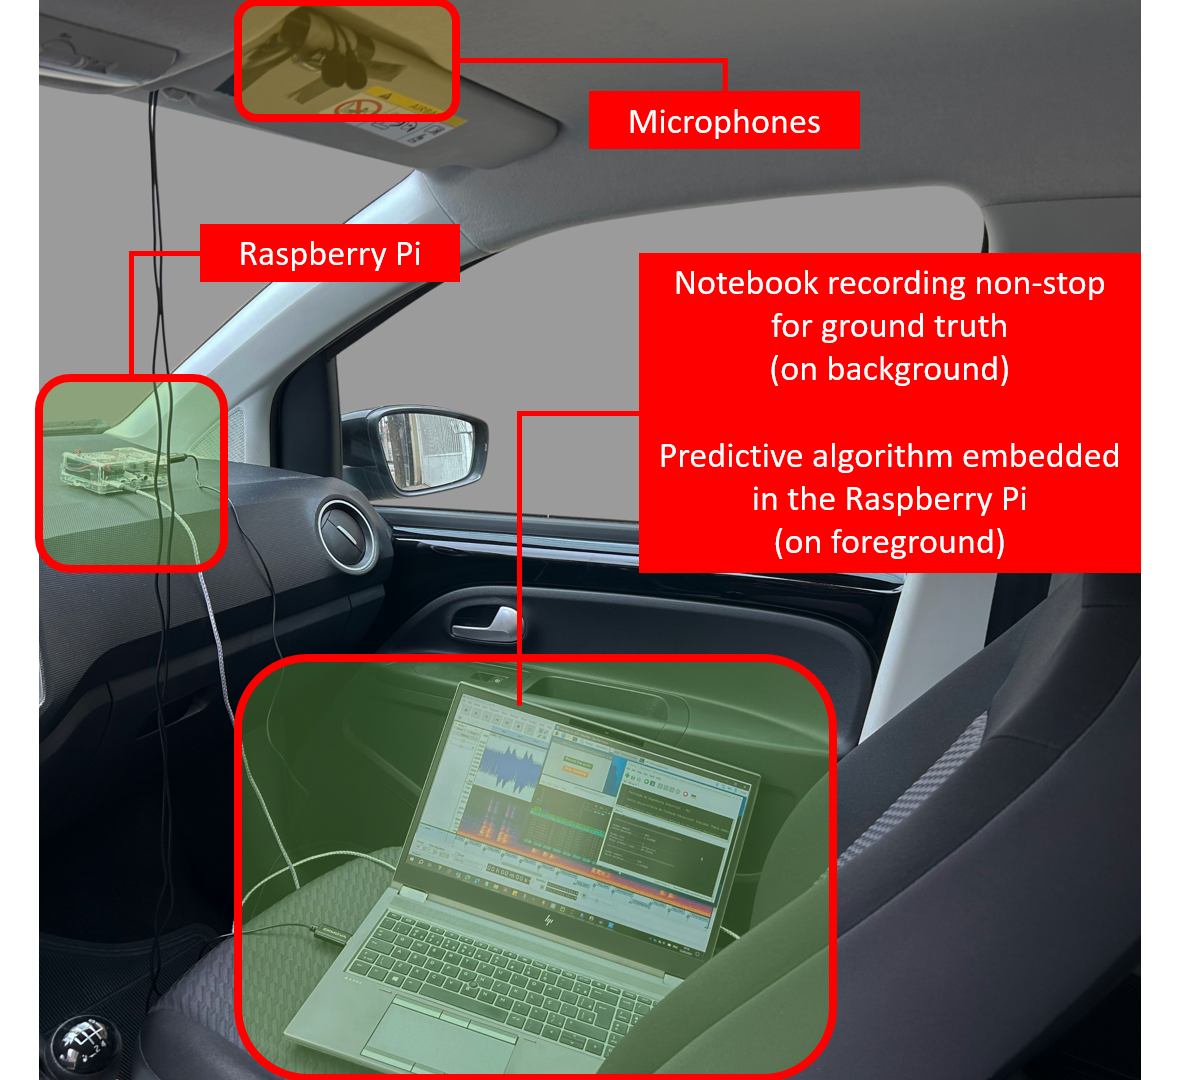
\includegraphics[width=.8\textwidth]{resources/images/050-methods/Methods_evaluation_outdoor.png}
        \smallcaption{Source: Author}
        \label{fig:methods_evaluation_outdoor_experiment}
\end{figure}